% !TEX root = ../main.tex

\chapter{LeverEdge: On-Chain Leveraged Tokens}\label{ch:leveredge}

\textit{This chapter is based on the work "LeverEdge: On-Chain Leveraged Tokens" supervised by Dr. \supv and submitted for comment to Financial Cryptography and Data Security 2025.}

\section{Introduction}
In this chapter, we provide a summary of our research focused on the design and proposal of LeverEdge, a fully decentralized leveraged token that addresses the deficiencies outlined in Chapter \ref{ch:shortfall}. As mentioned, Leveraged Tokens (LVTs) have been available to investors since 2019. They are often perceived as less risky than other forms of leveraged trading. However, recent research has identified ten critical deficiencies in the current offerings, primarily due to the lack of a standardized implementation framework. In this chapter, we review these shortcomings and explore potential solutions. To this end, we focus on several research questions and propose a new design model, LeverEdge, supported by a prototype deployed on the Ethereum blockchain. 

Unlike existing centralized and semi-centralized implementations, LeverEdge is fully decentralized and relies solely on-chain. This approach resolves most deficiencies, but operating fully on-chain is non-trivial because of the inherent complexities and limitations of blockchain technology, such as higher latency, scalability issues, and gas fees, especially when compared to the faster and more straightforward operations of centralized counterparts. As a result, we had to develop a new L1-L2 hybrid model which may be of independent interest. LeverEdge passed security checks and can serve as a potential reference model for future leveraged token deployments on EVM-compatible chains.

\section{LVT Return Dynamics}\label{appx:return}
A distinctive feature of the current decentralized LVTs is the variation in daily returns calculations. Let \( R_{t_{(n-1)\to n}} \) denote the return of a \(k\)-times LVT when the underlying price \( S \) fluctuates between times \( t_{n-1} \) and \( t_n \) (\(n \ge 1\)). Assuming zero daily interest expense and borrowing rate for simplicity, daily return is typically calculated as Equation (\ref{eq:return1}). In contrast, some LVTs employ an alternative power function, as shown in Equation (\ref{eq:return2}), leading to non-linear return dynamics.

\noindent
\begin{minipage}{0.5\linewidth}
	\begin{equation}
		R_{t_{(n-1)\to n}}=1+k\Big(\frac{\Delta S_{t_{n}}}{S_{t_{n-1}}}\Big) \label{eq:return1}
	\end{equation}
\end{minipage}
\begin{minipage}{0.5\linewidth}
	\begin{equation}
		R_{t_{(n-1)\to n}}=\Big(1+\frac{\Delta S_{t_{n}}}{S_{t_{n-1}}}\Big)^k \label{eq:return2}
	\end{equation}
\end{minipage}

\begin{figure}[t]
	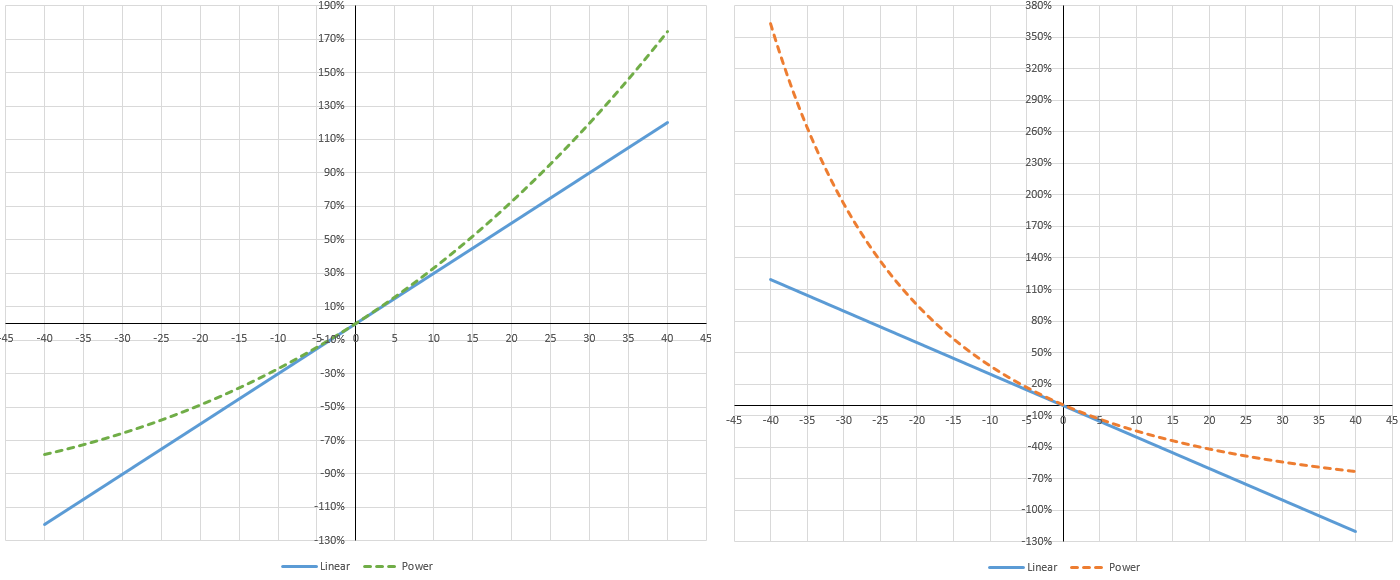
\includegraphics[width=\textwidth,keepaspectratio]{return.png}
	\caption[LVT return dynamics]{The return of a 3x LVT in response to changes in the underlying asset's price is characterized as follows: The return described by Equation (\ref{eq:return1}) follows a linear pattern (blue lines), while the return in Equation (\ref{eq:return2}) follows a power function (green and red dotted lines). The \(x\)-axis represents the percentage return of the underlying asset, and the \(y\)-axis denotes the return factor of the LVT. The returns of long and short tokens are illustrated in the left and right diagrams, respectively. In Equation (\ref{eq:return2}), the negative \(k\) for short tokens amplifies positive returns when the underlying asset's price experiences a sharp decline, leading to the return discrepancy between long and short tokens. This divergence may not be ideal for all users.}
	\label{fig:return}
\end{figure}

As illustrated in the dotted lines of Figure \ref{fig:return}, Equation (\ref{eq:return2}) amplifies the return of LVT compared to the linear behavior of Equation (\ref{eq:return1}), especially when the underlying price decreases and \(k\) takes more negative values. This is because the negative exponent enhances the return when the base (\ie change in the underlying price) is negative. This resulting in a larger positive return for short positions compared to long ones. For small changes in the underlying price (e.g., approximately less than 10\% when \(k = 3\)), both equations yield almost identical results, as the primary difference remains negligible for such small fluctuations. However, as the change in the underlying price becomes more significant, the returns from the two equations diverge sharply. This can result in varying financial outcomes for long and short positions.

\section{Evaluating Decentralized LVTs}\label{sec:evaluation}
As summarized in Table \ref{tab:solutions}, seven of ten deficiencies can be overcome by deploying the token on the blockchain. Therefore, decentralization should be considered as the primary approach, since the future centralized tokens is likely to suffer the same drawbacks. The remaining three issues relate to the functionality of the token itself, that can be addressed by optimizing internal algorithms. In this section we focus on on-chain LVTs, where some advances has already been seen. We further examine these tokens and assess the extent to which the identified issues are mitigated.

\ExecuteMetaData[sections/tables]{tab-solutions}

\subsection{FLI Tokens}\label{subsec:fli}
Index Coop launched FLI tokens in 2021 based on the Sets protocol~\cite{FLI_Sets}. These ERC-20 tokens consist of 4 smart contracts on the Mainnet and 6 on the Arbitrum blockchain. Tokens on the Mainnet and Arbitrum offer exposure to BTC and ETH up to 2x and 3x, respectively. Unlike most LVT issuers that create leverage through perpetual futures, FLI tokens directly use the lending market to create an over-collateralized leveraged position. While the FLI tokens are a step forward in decentralizing LVTs, it appears that they need optimization in some aspects:
\begin{enumerate}[label={\ref{subsec:fli}.\arabic*},leftmargin=*]
	\item \textit{Usability constraints:} FLI tokens may face usability issues due to supporting only ETH and BTC. Inverse and 3x tokens are available only on Arbitrum. Mainnet tokens have only 2x long exposure, and it is not possible to short BTC or ETH. Furthermore, U.S. residents are prohibited from buying these tokens~\cite{FLI_Restricted}. FLI tokens also has a \textit{Supply Cap} that in the past drove token prices higher~\cite{FLI_Shortage}.
	
	\item \textit{Fee impact:} Resorting to the debt market involves the payment of interest on the value borrowed. FLI also imposes transaction fees through swapping USDC against BTC/ETH. These costs are in addition to the 3.65-5.48\% management fee that may reduce the token return.
	
	\item \textit{Rebalancing risk:} Given that rebalancing involves constant price monitoring, FLI taps into off-chain servers for tracking leverage conditions before initiating the rebalancing process. Even though Index Coop uses a network of redundant servers for resilience, it still creates a single point of failure if issues arise with the company or all its servers become unreachable. Moreover, its \textit{Re-centering Speed} needs to be dynamically adjusted by market volatility for an optimal balance between tracking error minimization and rebalancing cost control.
\end{enumerate}

\subsection{Contango Tokens}\label{subsec:contango}
Contango protocol is developed by a team incubated by Alpha Venture in 2021~\cite{Contango_Blog}. It utilizes the lending and spot markets to generate leveraged positions through Automated Stacking and Flashswap. Users open new positions by depositing collateral into the Contango protocol. The operating contract posts collateral (ETH) on a lending platform (Aave, Compound), borrows another asset (USDC) against it, swaps it for the original asset (via Uniswap, Paraswap), and repeats the process over multiple loops to increase exposure. The high costs associated with executing these loops are minimized by Flashswap, enabling desired leverage in a single atomic transaction.

The protocol automatically mints an ERC-721 NFT whenever a user opens a new position. The NFT encapsulates details such as the underlying asset, leverage ratio, borrowing rates, and collateral. The designers claim that the implied funding rates for these positions are 2-3 times lower compared to traditional perpetuals. Volatility of the funding rate is also 2-4 times less,  making Contango a relatively attractive alternative~\cite{Contango_Doc,Contango_Medium}. Despite these advantages, Contango comes with certain limitations:

\begin{enumerate}[label={\ref{subsec:contango}.\arabic*},leftmargin=*]
	\item \textit{NFT transferability:} Secondary market for NTFs may face a lack of liquidity due to the specific features of each position: leverage, trading pair, lending market, and chain. As a result, liquidation of NFTs can be done only through smart contracts, which may leads to low trading volumes, market fragmentation, and high price volatility~\cite{seyhan2023nft}.
	
	\item \textit{Lack of liquidation protection:} To extend liquidation point, LVTs rebalance the fund automatically in case of sharp price swings. Contango, on the other hand, relies on users to actively monitor and manage positions manually to prevent liquidation~\cite{Contango_Faq}. This activity directly contradicts one of the key value premise of LVTs: simplifying position management. If a user is inactive or adjusts the position late, it could result in notable losses.	
	
	\item \textit{Multisig control:} Contango is not fully immutable; its core team is still capable of upgrading the smart contracts through a 3-of-5 multisignature process. This may introduces centralization risks.
	
	\item \textit{Liquidity risks:} During periods of market volatility or when liquidity is poor, slippage may increase in DeFi spot or lending markets~\cite{chiu2023fragility}, making it harder to execute trades or close positions at favorable prices.
	
	\item \textit{Variable borrowing costs:} Although Contango fees are typically much lower than those in traditional perpetual contracts, relying on variable-rate lending markets can cause borrowing costs to fluctuate. It may potentially resulting in higher-than-expected costs during periods of market volatility.
\end{enumerate}

\subsection{Cube Tokens}\label{subsec:cube}
Charm Finance launched Cube tokens in 2021 based on \textit{Parimutuel Pool} concept.\anote{parimutuel} Users deposit ETH into a smart contract, CubePool, to mint Cube tokens. These tokens can later be burned to withdraw the equivalent amount of ETH. The Cube token's value dynamically changes due to the underlying prices, pulled from Chainlink price feeds. While attempts at mitigating front-running and minimizing tracking errors through continuous rebalancing are in place, the current design falls short of meeting investor expectations on the following grounds:
\begin{enumerate}[label={\ref{subsec:cube}.\arabic*},leftmargin=*]
	\item \textit{Unequal profit distribution:} The return of LVTs is generally derived from the performance of the fund. In Cube, however, there is no fund—there are only losers paying winners, resembling a poker game where players compete for a shared prize or pot.
	
	\item \textit{Inaccurate leverage tracking:} Due to the normalization process, Cube tokens do not accurately track the leverage, making them unsuitable for investors seeking precise returns.
	
	\item \textit{Disincentive for large investments:} Those holders who have large pool ownership earn the least profit because of losses incurred during the normalization, while owners with smaller pool shares experience fewer losses. This dynamic discourages large investments, making them economically unjustified.
	
	\item \textit{Elevated performance risk:} Performance of Cube tokens is relative to each other. For instance, if Bitcoin goes up by 1\%, the owner of BTC tokens may still lose value if other tokens in the pool have increased by a greater amount.
	
	\item \textit{Leverage dilution:} When too many users buy the same token, its leverage can decrease, potentially dropping below 1x or even turning negative.
	
	\item \textit{Hindered token adoption:} The safety mechanism of CubePool sets the limit on the Total Value Locked at 100 ETH. When this limit is reached, users cannot buy tokens until others sell~\cite{Cube_Github}. This may limit token usability.
	
	\item \textit{Management risk:} Each pool maintains two super accounts, namely: Governance and Guardian. They have the privilege to execute emergency ETH withdrawals and to pause/unpause pool operations~\cite{Cube_Faq}. This kind of centralization may not precisely meet the risk appetite of some investors.
\end{enumerate}

\subsection{Squeeth Tokens}\label{subsec:squeeth}
In 2021, Opyn launched Squeeth token (oSQTH). It offers nearly 2x exposure to ETH's volatility. Users can mint it via Opyn's app or trade it for ETH on DEXs~\cite{Squeeth_Doc}. However, oSQTH may face the following challenges in adoption:
\begin{enumerate}[label={\ref{subsec:squeeth}.\arabic*},leftmargin=*]
	\item \textit{Volatility speculation:} Squeeth's payoff is non-linear and tracks \( \text{ETH}^2 \). This feature increases sensitivity to changes in the ETH price as shown in Figure \ref{fig:return}. oSQTH acts more as of a proxy for ETH volatility, and traders holding them speculate on price movement "patterns" rather than directly on the underlying asset's price. This contrasts with the expected linear return of LVTs~\cite{Squeeth_Medium}.
	
	\item \textit{Premium costs:} The daily funding fee in most of the perpetual futures is 0.03-0.05\%~\cite{Coinglass_Funding}, while users pay a 0.1-0.5\% premium in Squeeth to benefit from higher risk-to-reward ratio~\cite{Squeeth_Funding}. As shown in Figure \ref{fig:return}, its power function return works in favor of users in volatile markets. It is worth mentioning that if the price of crypto-asset remains flat for an extended period—something that happens about 50-60\% of the time~\cite{bulkowski2011encyclopedia,edwards2007technical}—returns can be significantly eroded due to this heightened funding premium.
	
	\item \textit{Complexity:} To counter token value inflation, Squeeth undergoes regular normalization. Additionally, short positions require users to post collateral to hedge against volatility risk, while this is not required for long positions. Moreover, oSQTH is not available to U.S. persons and certain residents of 15 more countries~\cite{Squeeth_Restricted}. These factors add complexity, especially for traders unfamiliar with the specific mechanics of trading Squeeth token.
\end{enumerate}

\ExecuteMetaData[sections/tables]{tab-toros}

\subsection{Toros Tokens}\label{subsec:toros}
Toros Finance issued Toros tokens in 2023 on L2 chains (see Table \ref{tab:toros} for the list of supported tokens). These tokens use different smart contracts from dHEDGE, Aave, and 1inch to automate both leverage and asset management. The system, while decentralized in nature, still suffers from some limitations:

\begin{enumerate}[label={\ref{subsec:toros}.\arabic*},leftmargin=*]
	\item \textit{Usage constraints:} With the view to minimize transaction costs, Toros tokens are deployed solely on L2 chains, which results in restricted access to greater liquidity available on the Mainnet. Moreover, trading flexibility is limited as usually only ETH and BTC are supported across all L2 chains.
	
	\item \textit{Transparency risks:} The absence of token contract code on the blockchain for specific tokens can result in reduced adoption and create security risks since auditors are unable to confirm the token's functionality.\anote{TorosETH}
	
	\item \textit{Upgradability risks:} Toros tokens can be upgraded~\cite{Toros_Doc}, adding complexity and resulting in increased gas costs because of the proxy pattern used. This ability to upgrade also brings security risks if admin control is ever compromised. Additionally, it raises concerns about possible changes to the fundamental logic of the token.
	
	\item \textit{Manual rebalancing:} The rebalancing process in the dHEDGE protocol (and by extension, Toros) is not automated or on a fixed schedule. dHEDGE offers manual rebalancing, enabling fund managers to modify their positions according to their strategies and market conditions~\cite{dHEDGE_Design}. Nevertheless, this method comes with the potential drawback of experiencing delayed rebalancing in unpredictable markets, which could harm overall performance. Additionally, novice users may not have the appropriate resources to adequately track prices and react promptly, which could heighten the risk of incurring significant losses.
\end{enumerate}

\subsection{TLX Tokens}\label{subsec:tlx}
TLX tokens were introduced in 2024, offering up to 20x leverage exposure to more than 50 assets. Every token is supported by Synthetix Perp v2 futures. Individuals have the option to deposit either USDC or sUSD\anote{sUSD} and choose their desired asset, leverage, and trading direction. The procedure involves creating TLX tokens that can be exchanged for USDC or sUSD at a later time~\cite{TLX_Doc1,TLX_Doc2}. To gain wider market acceptance, TLX tokens might need some optimizations:
\begin{enumerate}[label={\ref{subsec:tlx}.\arabic*},leftmargin=*]
	\item \textit{Chain restrictions:} The limitation of TLX tokens to the Optimism network hinders users from accessing it on other L2 chains. Moreover, individuals familiar with the Mainnet or other L2 alternatives might experience decreased liquidity and may not perceive a benefit in transitioning to Optimism, resulting in less usability.
	
	\item \textit{Synthetix v2 limitations:} Presently, TLX tokens are dependent on Synthetix v2, therefore requiring an upgrade to Synthetix v3. Staying connected to the outdated version could leave the protocol vulnerable to risks of updates.
	
	
	\item \textit{Leverage imbalance:} The different leverage ratios of [1.87x-2.18x] for 2x long and [1.61x-2.53x] for 2x short tokens create an uneven risk exposure. The inconsistency in leverage is widespread among all TLX tokens, making it challenging for traders to keep balanced hedging strategies.
	
	\item \textit{Audit concerns:} The audit report expresses concerns about off-chain rebalancing signals, as well as risks associated with liquidation, immutability, and treasury exposure~\cite{TLX_Audit}.
\end{enumerate}

Even though there have been notable attempts to decentralize LVTs, a closer look at their functionality shows ongoing shortcomings that need to be addressed. In this regard, we propose and evaluate a new L1-L2 hybrid model, LeverEdge, and compare how well it performs against others. As shown in Table \ref{tab:compare}, LeverEdge addresses most of the existing problems and also brings additions like front-running alleviation and lowered fees.

\ExecuteMetaData[sections/tables]{tab-compare}

\section{LeverEdge: New Proposal}\label{sec:proposal}
\subsection{Leveraged Product Selection}\label{subsec:selection}
Our research highlights three possible choices for leveraged products in creating a fund for LVTs: (i) futures contracts, (ii) leveraged positions based on debt, and (iii) synthetic assets. Although the debt market may have lower and more consistent funding rates, perpetual contracts offer unique benefits such as easy access to both long and short positions and efficient rebalancing.

The selection of leveraged products involves various important factors: Firstly, LVTs are designed for experienced traders who have a thorough understanding of market dynamics. They generally focus on immediate price changes rather than long-term holding strategies. Day traders face one of two outcomes: either the price trend matches their initial analysis, enabling them to make a profit within the same trading day, or the analysis proves to be incorrect, leading to a swift exit to reduce losses. They do not stay in positions for an extended amount of time to take advantage of the reduced costs in debt-based LVTs. Additionally, they are aware that if the market goes against them, the probability of a positive turnaround on the same trading day is slim~\cite{fung2000intraday}. As a result, LVTs are specifically made for skilled traders, with inexperienced users being more prone to losses, if they hold LVTs for a long time. 

The second important factor riles on the fact that, the debt market is not efficient for establishing short positions. Lending protocols usually demand that stablecoins be over-collateralized in order to borrow crypto-assets at a 1:1 ratio. Creating short tokens is less lucrative and more difficult than creating long positions (see Figure \ref{fig:looping} and compare the processes of creating long and short positions). This assertion is additionally supported by Table \ref{tab:compare}, demonstrating that debt-based LVTs solely provide -1x short tokens, not leverages like -2x, -3x or -5x. Having this restriction limits the capacity to form short positions that are similar to long ones.\anote{inverse} Given these constraints in the lending market, our design is (i) structured around perpetual futures rather than the debt market, (ii) more suitable for short-term traders.

\begin{figure}[p]
	\centering
	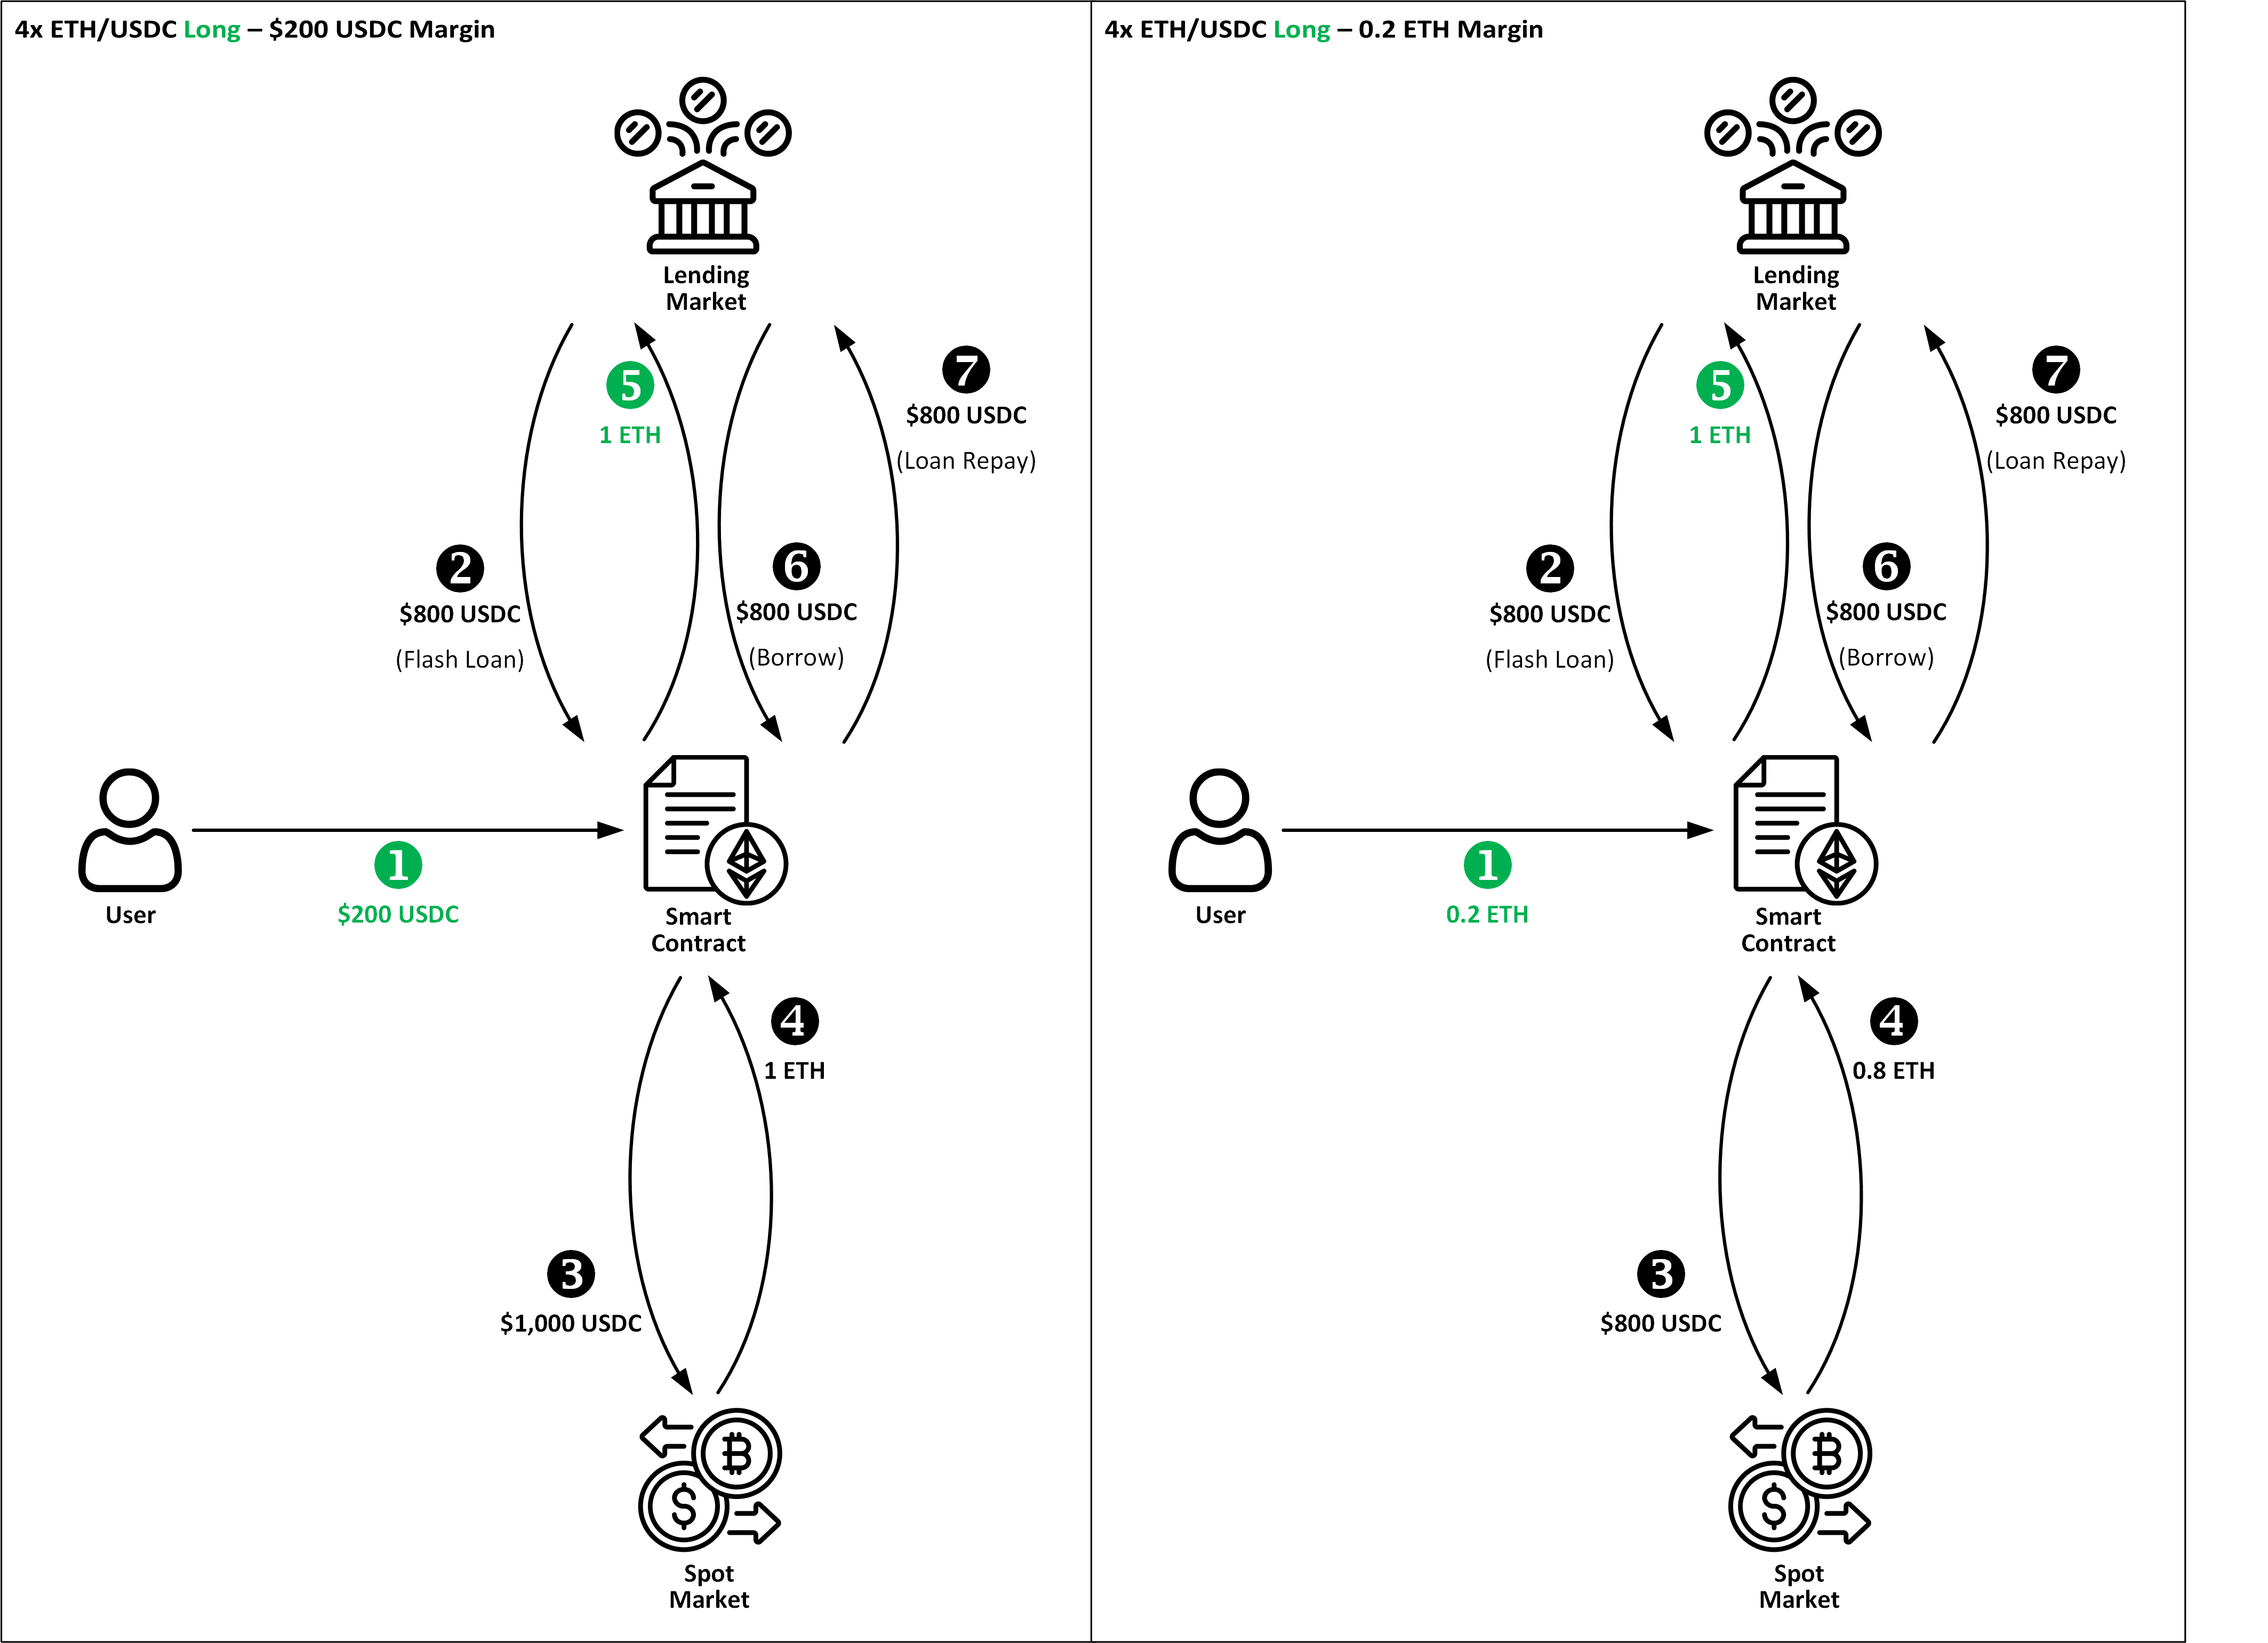
\includegraphics[width=0.9\textwidth,keepaspectratio]{long.png}
	\caption[Long vs. Short Position Creation]{Diagrams illustrating the creation of a 4x long (top) and short (bottom) position through automated looping, where users either deposit stablecoins (left) or post crypto as margin (right). Short positions differ from long positions in that they require full exposure to the notional value of the asset being shorted.}
	\centering
	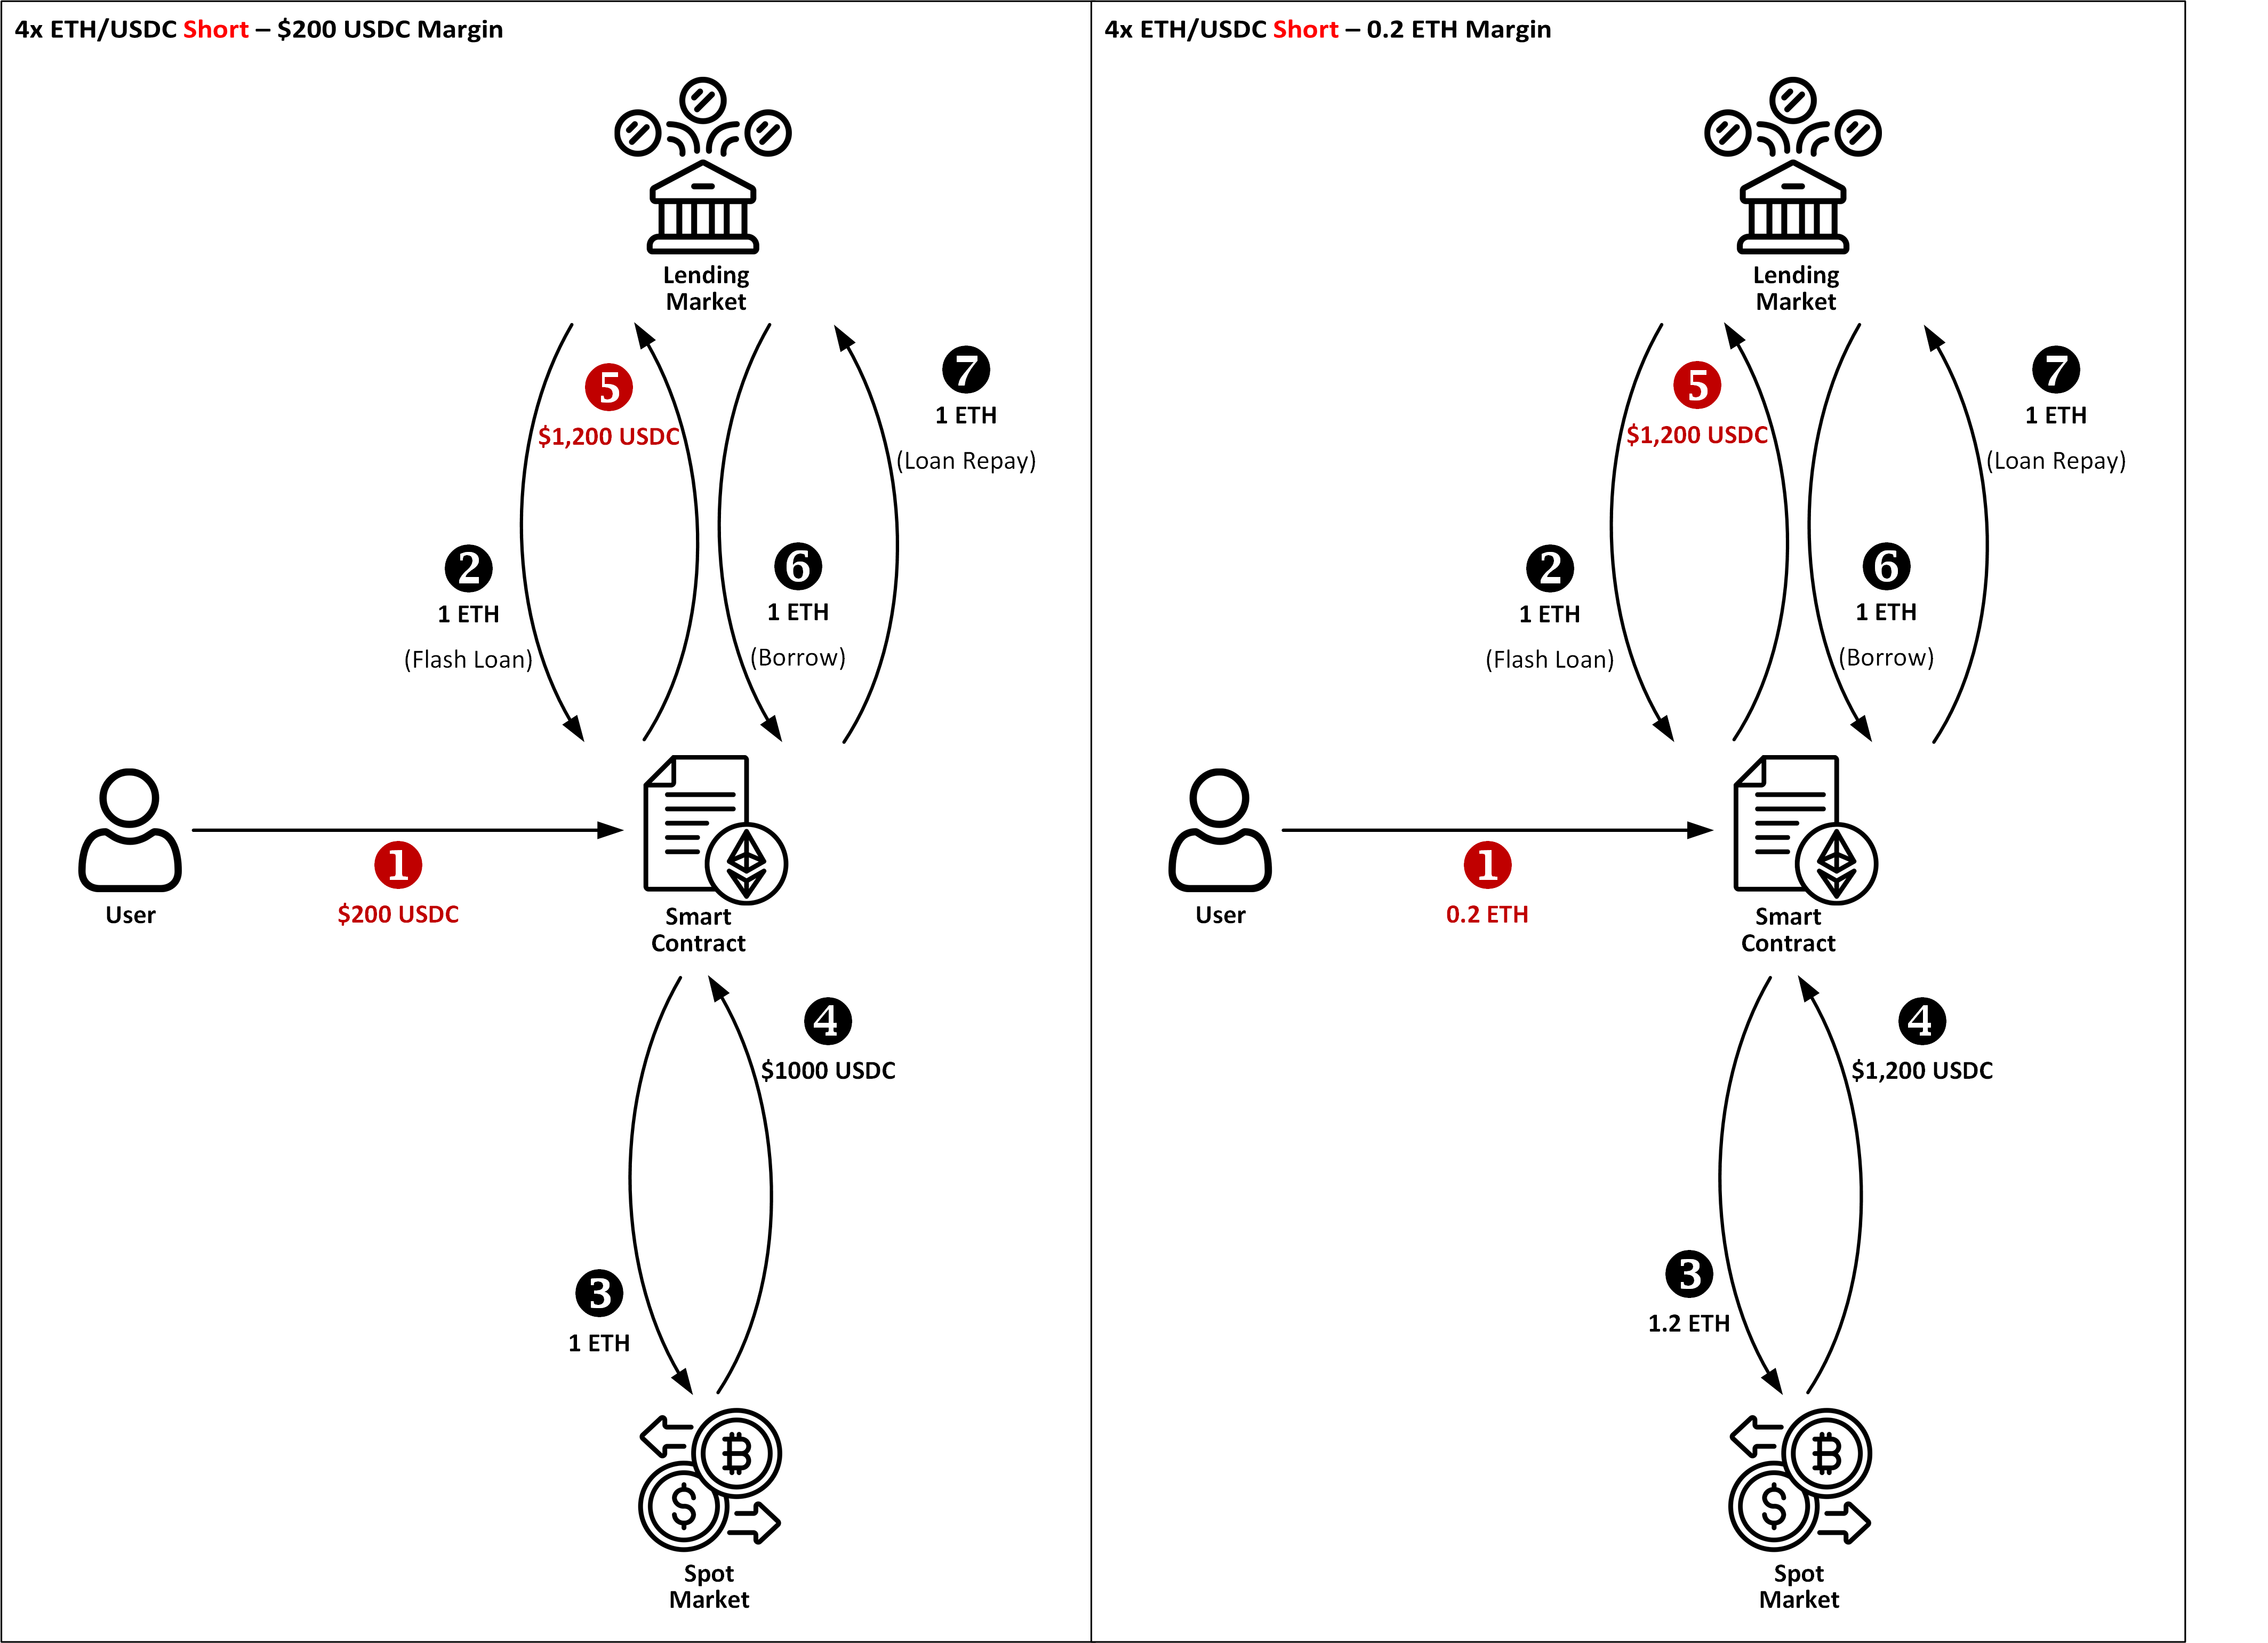
\includegraphics[width=0.9\textwidth,keepaspectratio]{short.png}
	\label{fig:looping}
\end{figure}

\subsection{Resolving LVT Shortcomings}\label{subsec:resolve}
Mentioned risks affect the financial efficiency and reliability of LVTs, leading to less acceptance by investors. Implementing LVT on the blockchain can address these issues by bringing transparency to the total supply, transactions, holders, custody, auditing and financial backing. On-chain implementation should therefore be used by LVTs to mitigate the associated risks in centrally issued tokens.

Another discussed issue is the effect of front-running which may place LVT in a position where it needs to execute more trades than otherwise required for simple rebalancing (see Section \ref{subsec:frontrunning} for more details). Front-running has always been a challenge in traditional markets, but most issues have been controlled through regulatory oversight~\cite{SEC_Oversight}. Lacking that regulation in crypto, the risk can be mitigated by: (i) camouflaging trading intent through enhanced algorithms that randomize both the timing and size of rebalancing trades, making it harder to predict when and how much of the underlying asset will be bought or sold; (ii) cross-trading between long and short pairs, whereby issuers internally swap matching positions to minimize the need for open market transactions, as token issuers can act as the LP and match orders for different LVTs in-house; and (iii) collaborating with liquidity providers and market makers (\eg permissioned pools by Aave Arc and Fireblocks~\cite{Aave_Arc}), allowing issuers to discreetly source liquidity and execute large orders without revealing their trading intentions.

Although we proposed solutions for front-running, there would be still a possibility of front-running by miners who may intentionally include the rebalancing transaction in upcoming blocks and delay it to prioritize their own. Therefore, the risk of front-running can be alleviated and not completely eliminated.

A further issue with LVTs is tracking error (leverage deviation). Some of the ways to reduce tracking error include: (i) increasing rebalancing frequency, possibly every \(n\) blocks instead of the default daily rebalancing, to more precisely maintain the target leverage ratio. This may involve using L2 chains that have lower transaction fees; (ii) performing interim rebalancing at threshold crossings of the underlying asset price (\eg \(\pm10\%\)), which would mitigate the impact of sudden price changes by rebalancing leverage more than once a day; and (iii) having a range allowing variation in leverage (\eg [1.95x, 2.05x] for a 2x long token), permitting small deviations without rebalancing. Thus, for both long and short tokens, this range must be set carefully to avoid major tracking errors. This approach should also be fully explained to investors to manage expectations properly, as it represents a workaround rather than a definitive solution.

Another notable difference in LVTs is high management fees compared to LETFs that can be minimized by: (i) using advanced algorithms (iceberg or reverse orders), which enable the optimization of the timing and size of trades to minimize slippage and bid-ask spread costs; (ii) cross-trading between long and short funds, since issuers operating both can internalize trades by directly matching orders of funds sharing the same underlying assets. This internal matching at better prices further reduces slippage and transaction costs; (iii) using L2 chains~\cite{Gangwal_2022} in combination with MultiCall transactions~\cite{hughes2021multicall}, which further lower the operating cost.

\begin{figure}[t]
	\centering
	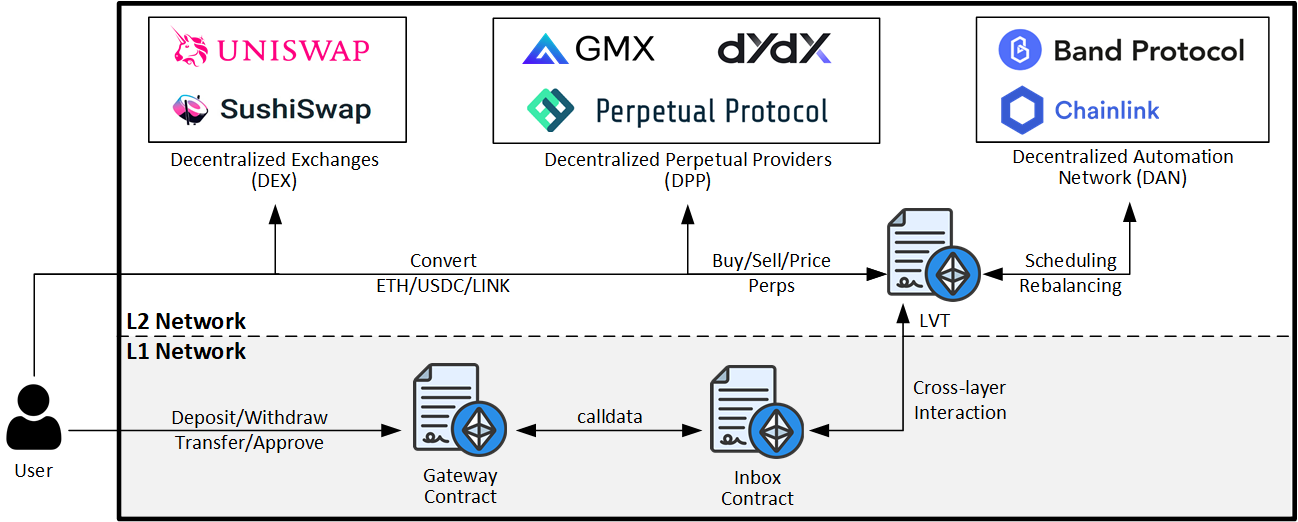
\includegraphics[width=\textwidth,keepaspectratio]{design.png}
	\caption[LeverEdge components: DEX, DPP, DAN, and gateway]{The core components of LeverEdge consist of the DEX, responsible for handling necessary crypto exchanges. Futures positions are managed via DPP, while the rebalancing process is triggered by DAN. Users can interact directly with the token on L2 or rely on the gateways contract, which streamlines cross-layer contract interactions.}
	\label{fig:design}
\end{figure}

\subsection{Design Model}
LeverEdge follows a hybrid L1-L2 architecture, with smart contracts deployed on both L1 and L2 chains. The L2 contract acts as the primary code, managing the core functionality of the token. Users can directly interact with the L2 contract if their funds are already on L2, or they can access the token via the gateway contract on L1, which accepts funds and facilitates communication with L2 (see cross-layer interaction in Figure \ref{fig:design}). The gateway contract serves as the main entry point for L1 users, enabling interaction with L2 through Bridge or Inbox contracts. Thus, user-facing operations in LeverEdge can occur on either L1 or L2, depending on where users hold their funds, while trading activities remain on L2 to ensure faster, more cost-efficient execution. This hybrid architecture optimizes scalability and security by allowing the L1 contract to handle secure finality, while L2 focuses on high-speed execution and cost reduction.

LeverEdge design allows issuers to choose DeFi partners according to factors like service fees, security, and performance. As shown in Figure \ref{fig:design}, it incorporates three main groups of DeFi providers: (i) DEX for trading crypto assets on-chain, (ii) DPP for establishing leveraged positions with perpetual contracts, and (iii) DAN for monitoring conditions and executing smart contract functions upon meeting predetermined criteria, such as daily or interim rebalancing.

\begin{example}
	A LVT issuer may decide to use Uniswap instead of Sushiswap for making a 2x long ETH token (ETH2L), while another might select GMX on Arbitrum rather than dYdX on StarkEx for handling perpetual futures. dYdX appeals to high-volume traders with its gasless trading, whereas GMX attracts retail traders with its higher leverage options. Ultimately, both tokens deliver twice the yield of ETH, but through different DeFi services: the first approach reduces token operating costs, while the second prioritizes user adoption.
\end{example}

The process of incorporating DeFi services into LeverEdge is made more efficient with standardized interfaces. LVT issuers can choose their preferred DeFi partners without impacting the token's primary functions. Essentially, LeverEdge creates interfaces that encapsulate DeFi services, enabling the token to function smoothly with various providers, regardless of their internal procedures.

\subsubsection{Decentralized Exchange (DEX)}
Most DeFi systems use USDC as the primary transaction currency, and LeverEdge operates seamlessly with it. It accepts USDC by default while also supporting ETH-to-USDC conversion. If users send ETH to the contract, it is automatically converted to USDC. Similarly, when users sell tokens, they can choose to receive either USDC or ETH. Interacting with LeverEdge using USDC minimizes conversion fees. In line with a fundamental principle of blockchain, the requester is responsible for paying all associated fees. This means that users initiating buy or sell transactions are required to cover all relevant costs, including any fees for converting USDC to ETH.

In addition to USDC, LINK tokens are required to automate certain tasks. These tokens are consumed by the Chainlink network to trigger the rebalancing process. During each rebalancing event, a portion of the perpetual contracts are sold and converted from USDC to LINK, which is then sent to Chainlink as an incentive to maintain the rebalancing mechanism. 

Interaction with decentralized exchanges is essential for LeverEdge to handle both internal and external currency conversions. By default, Uniswap is used due to its lower exchange fees and higher liquidity. However, the modular design of LeverEdge allows for integration with other DEX providers, such as Sushiswap, Paraswap and Kyberswap.

\subsubsection{Decentralized Perpetual Provider (DPP)}
Decentralized perpetuals offer a decentralized alternative to dominant centralized platforms, allowing LeverEdge\ to create long or short exposure to various crypto assets. When it comes to decentralized perpetuals that can only be traded on L1, the options are relatively limited due to scalability constraints and high gas fees. The more viable solution is to use DPPs on L2 networks such as Polygon, Optimism, Arbitrum, and StarkNet. However, there is a need to make communication between L1 and L2 seamless to improve the user experience. In this regard, we implement a gateway contract on L1, which facilitates user interaction with L2. 

Users do not need to bridge their funds manually, as the gateway contract handles this process for them. The gateway contract works in conjunction with the bridge contract of the corresponding L2 chain, enabling LeverEdge\ to securely transfer user assets between the two layers while maintaining decentralization and security. The gateway contract also communicates with the main contract on L2 through a messaging system. The primary mechanism for transferring data between L1 and L2 involves sending messages via LeverEdge smart contracts deployed on both layers.

dYdX and GMX are two popular DPP platforms on L2 that can be integrated with LeverEdge. On dYdX, USDC is the only accepted collateral, and all deposits must be made in USDC. dYdX has migrated its perpetual v3 trading entirely to the StarkEx L2 chain. StarkEx, utilizes zk-rollups to enhance transaction throughput and minimize gas fees. It uses StarkEx to settle perpetual contract trades on its platform, offering a more efficient and scalable trading experience while maintaining security by relying on L1 for data availability. dYdX has implemented the \textit{Currency Converter} and \textit{StarkEx Bridge} contracts on L1, which LeverEdge uses to communicate with the main dYdX contract on L2.

\begin{example}\label{ex:experience2}
	Alice deposits \$100 USDC from Ethereum L1 into the ETH2L token, which is configured to use GMX on Arbitrum. Instead of sending USDC directly to the main ETH2L contract on the Arbitrum network, Alice sends her USDC to the ETH2L gateway contract on L1. The gateway contract then interacts with the Arbitrum Bridge contract deployed on L1 to transfer Alice's \$100 USDC to the main ETH2L contract on Arbitrum. Additionally, the gateway contract appends metadata to the transaction, linking the deposited funds on Arbitrum with Alice's L1 address.
\end{example}

LeverEdge allows seamless selection of providers due to the modular design of the DPP contract. This decouples the internal mechanics of each provider. The DPP contract implements the \texttt{buyPerp()} and \texttt{sellPerp()} functions to interact with DPP. These functions are called by the \texttt{subscribe()} and \texttt{redeem()} methods for buying and selling futures. Since the internal buy or sell logic is abstracted away from these methods, token issuers can select the appropriate DPP when initially creating tokens.

LeverEdge\ supports cross-layer contract interaction, where it sends a transaction from L1 that not only bridges the funds but also triggers a function call on the main contract in Arbitrum. This is achieved using the \textit{Inbox} contract deployed on L1. The Inbox contract allows the passing of \textit{calldata}, which specifies the contract to call and the function to execute once the funds are deposited on L2. LeverEdge uses this mechanism to communicate with the main contract.

\begin{example}
	In the Example \ref{ex:experience2}, the L1 Bridge contract of Arbitrum locks Alice's USDC on L1 and generates a message sent to the L2 chain. This message is bundled into a batch of transactions that are eventually processed by L2, crediting the main ETH2L contract on Arbitrum. Conversely, when ETH2L sells GMX positions and withdraws funds from Arbitrum, the L2 chain sends a message to the L1 Bridge contract, which releases Alice's USDC after a challenge period (\ie one week in the optimistic rollup used in Arbitrum).
\end{example}

\subsubsection{Decentralized Automation Network (DAN):} Smart contracts cannot autonomously execute their functions based on predefined conditions or time. They require external triggers, either manual or via centralized mechanisms, both of which have significant limitations. Manual triggers are impractical, and centralized solutions are vulnerable to failure or exploitation. 

Decentralized solutions like Chainlink address this issue by enabling smart contracts to automate key functions. Chainlink provides a Distributed Automation Network (DAN) that continuously monitors predefined conditions, which may be based on time, events, computations, or a combination of these factors. Nodes within the Chainlink network initiate on-chain transactions once the conditions are met, triggering the smart contract’s functions. In LeverEdge, we use Chainlink to automate both regular and interim rebalancing processes.

\subsubsection{Modular Architecture}
LeverEdge is designed in a modular fashion by defining specific interfaces. These interfaces outline the required function signatures for inherited contracts without providing their implementation. By using interfaces, LeverEdge enables standardized interaction, fostering a modular and extensible contract architecture. Developers can create custom modules and integrate different providers with the token, as long as they adhere to the same interface specifications. This flexibility ensures seamless integration while maintaining compatibility across various components.

\begin{example}\label{ex:swap}
	The \texttt{swapEth()} method is designed to convert ETH to USDC, with the underlying DEX provider being either Uniswap or Sushiswap. From a functional perspective, the method’s sole purpose is to perform the conversion, regardless of the internal mechanism of the chosen DEX. If issuers are not fully satisfied with the service quality, they can select competing providers. Methods such as \texttt{setDexProvider()}, \texttt{setDppProvider()}, and \texttt{setDanProvider()} facilitate this flexibility, allowing issuers to specify providers when initially deploying the smart contract. 
\end{example}

If changing the provider does not impact the token's functionality, it can be performed even after token deployment. In Example \ref{ex:swap}, the switch from Uniswap to Sushiswap can occur live, without affecting the fund's value or futures positions. This transition ensures that Sushiswap handles the conversion instead of Uniswap, while maintaining the same currency conversion functionality. The issuer may plan this change to reduce costs or optimize the conversion process. Similarly, issuers can change the DAN live, as it triggers the rebalancing process at specific intervals.

\begin{figure}[p]
	\centering
	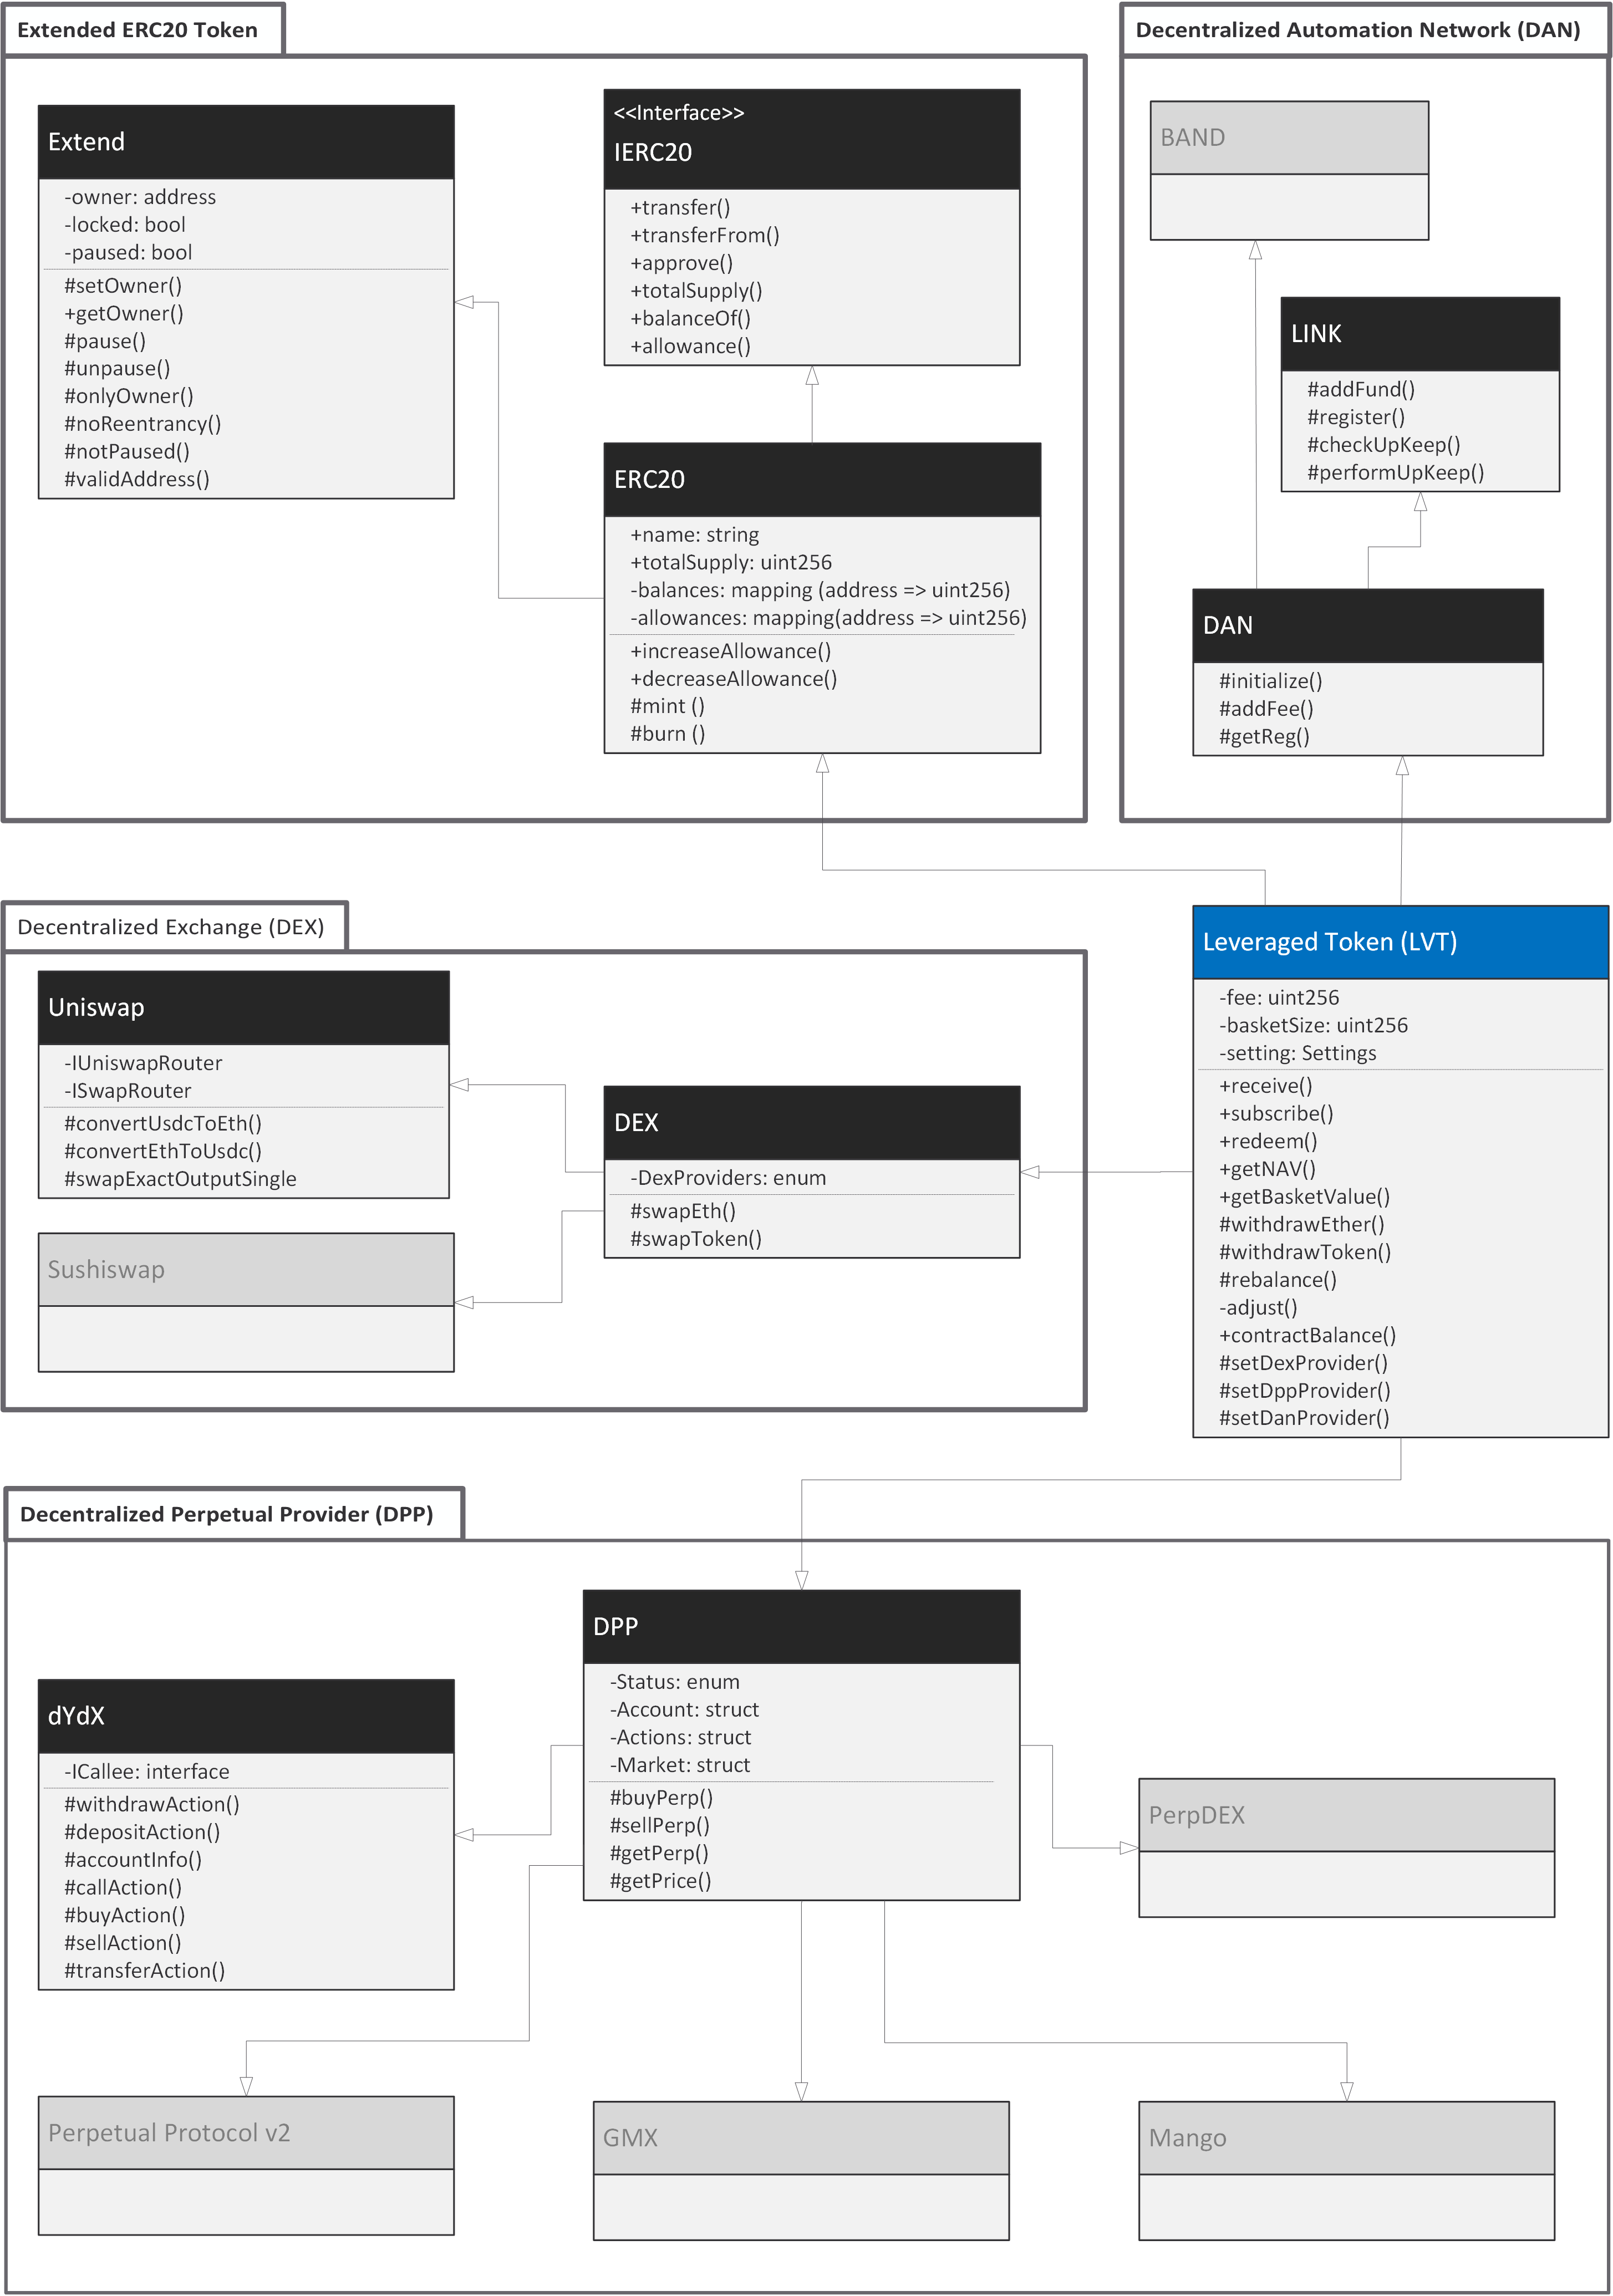
\includegraphics[width=0.85\textwidth,keepaspectratio]{model.png}
	\caption[LeverEdge design model]{The design model of LeverEdge, our proposed decentralized leveraged token, is presented as a UML class diagram. The LVT contract inherits from the ERC-20, DPP, DEX, and DAN contracts. Contracts marked in gray are not implemented and are included only to illustrate possible alternatives. For example, a developer might prefer to use GMX instead of dYdX in a custom implementation.}
	\label{fig:model}
\end{figure}

\subsubsection{Users Experience}
The initial token price is usually set at \$1, with a starting supply of zero tokens. As users deposit funds, the token supply increases proportionally. When users sell tokens, those tokens are removed from circulation, maintaining a dynamic supply that adjusts based on user activity. End-user interaction with the token begins by sending USDC or ETH to the \texttt{subscribe()} method. If users bypass this method and send funds directly to the smart contract address, they must later use the \texttt{claim()} method to receive the equivalent value in tokens. This mechanism addresses cases where funds are mistakenly sent to the smart contract without invoking the \texttt{subscribe()} method.

Upon receiving funds, the smart contract purchases futures aligned with the token's leverage. It calls the \texttt{buyPerp()} function from the DPP module to interact with the futures provider and increase contract positions. Atomic transactions ensure the consistency of the transaction. Whether it fails or succeeds, the transaction cost is incurred by the user initiating the new position. 

These newly acquired perpetuals directly impact the overall fund value, which can be validated by calling the \texttt{getBasketValue()} method. This method is usually called by auditors to ensure proper financial backing. Additionally, the number of contracts on the DPP can be directly verified, as each buy and sell transaction triggers a \texttt{BuyPerp} or \texttt{SellPerp} event logged on the blockchain.

\begin{example}\label{ex:experience1}
	Bob sends \$10K USDC to the \texttt{subscribe()} method of a 3x leverage token when the Bitcoin perpetual price is \$30K. As a result, \$30K worth of futures contracts are purchased and added to the fund value. The \texttt{subscribe()} method also invokes the \texttt{mint()} function of the smart contract to update Bob's token balance (refer to the ERC-20 interface in Figure \ref{fig:model}). Bob can later check his token balance by calling the \texttt{balanceOf()} method of ERC-20 interface.
\end{example}

\subsubsection{Net Asset Value}
The Net Asset Value (NAV) is typically used by users engaging in bulk transactions, as it reflects the token's true value. Throughout the trading day, the token price may fluctuate due to market volatility, resulting in a premium or discount. The NAV price can be retrieved using the \texttt{getNAV()} method, which calculates the actual price based on the underlying asset's value and the token's leverage, after deducting fees. The returned value, in USDC, serves as a reference for determining the token's fair value. 

It is worth noting that fees are automatically deducted daily, causing value of LeverEdge to gradually decrease relative to the futures it holds. This mechanism ensures that fees are paid from the token's total assets, reducing the NAV proportionally. Consequently, daily fee deductions impact the token's price over time, making it more suitable for short-term investments. In a prolonged sideways market, fees may reduce returns in buy-and-hold scenarios.

\begin{example}
	To sell tokens in the Example \ref{ex:experience1}, Bob can call the \texttt{getNAV()} method to get the NAV price he will receive. Then, he may invoke the \texttt{redeem()} method and specify the number of tokens he wishes to sell. The \texttt{redeem()} method calculates the equivalent USDC value and transfers it to Bob after selling the corresponding futures. Bob also incurs all necessary transaction fees when initiating the sale.
\end{example}

\subsection{Price Dynamics}
LeverEdge amplifies exposure to price movements of the underlying (the price of perpetual futures), both upward and downward. Let \( P_{t_n} \) represent the price of the \(k\)-times leveraged token at time \( t_n \). The token’s price evolves in response to changes in the underlying asset \( S_{t_n} \) between time \( t_{n-1} \) and \( t_n \). In continuous time, this price change can be described by a differential equation that incorporates: (i) token leverage, (ii) underlying price fluctuations, (iii) funding and management fees. The differential form of \(P_{t_n}\) is given by the following stochastic differential equation (SDE):
\begin{equation*}
	\frac{dP(t)}{P(t)} = k \frac{dS(t)}{S(t)} - \big(F(t) + M(t)\big)dt
\end{equation*}
Where the first term represents the leveraged return from the underlying perpetual futures (tracking asset), amplifying the token return by the leverage factor \(k\). \(F(t)\) is the continuous funding fee rate, typically expressed as a daily rate per second. It reflects the cost (or sometimes gain) of holding the perpetual futures during the given period. \(M(t)\) is the continuous management fee rate, expressed annually but calculated per second. By solving the SDE over the interval \([0, t]\), we obtain the continuous-time price formula:
\begin{equation}\label{eq:lvt1}
	P(t) = P(0) \cdot \exp\left( \int_0^t k \cdot r\big(S(\tau)\big) \, d\tau - \int_0^t \big( F(\tau) + M(\tau) \big) \, d\tau \right)
\end{equation}
Where P(t) is the value of the token (or NAV) at time \(t\). \(P(0)\) is the initial token price at time \(t=0\). The first term reflects the cumulative leveraged return of the underlying over the time period \([0,t]\). \(r\big(S(\tau)\big)\) is the return on the underlying asset \(S\). The second term accounts for the accumulated funding and management fees over the same period. In summary, equation \ref{eq:lvt1} expresses LeverEdge's price as a function of the underlying futures return, adjusted for continuously accruing funding and management fees. This formulation captures the real-time dynamics of LeverEdge's price evolution in response to market movements and the associated costs.

Since funding and management fees are usually expressed as daily or yearly rates, they can be discretized into small intervals (such as seconds or minutes) to approximate the continuous accrual process. This method ensures that fees are seamlessly integrated over time, preventing users from avoiding fees by timing their buy or sell actions just before daily fee deductions. In this regard, the following formula is used to calculate LeverEdge's price in discrete time between \( t_{n-1} \) and \( t_n \) for intraday token buy or sell transactions:
\begin{equation}\label{eq:lvt2}
	P_{t_n} = P_{t_{n-1}}\left(1+k\frac{\Delta S_{t_{n}}}{S_{t_{n-1}}}\right) \times \big(1 - (F_{t_n} + M_{t_n}) \big), \quad \forall \, t \ge 1
\end{equation}
\(M_{t_n}\) and \(F_{t_n}\) represent the management and funding fees, respectively. \(P_{t_n}\) is calculated based on the percentage change in the underlying asset \(S_{t_{n}}\). The deduction is incorporated into the token's price, meaning holders indirectly pay the fee as the token value is adjusted daily. There is no need for holders to manually send any funds; instead, the token’s value continuously reflects the deduction of the fee.

\begin{example}
	Alice deposits USDC into a ETH5L token at 7 a.m. when the token price is \$1 per token. She receives the equivalent ERC-20 tokens in return. By 11 p.m., the price of ETH has increased by 10\%. As a result, the ETH5L token rises by \(10\% \times 5 = 50\%\), reaching \$1.50 per token. This amplifies Alice's initial investment by a factor of \(k=5\).
	\begin{equation*}
		P_{11pm} = P_{7am}\left(1+5\frac{\Delta S_{11pm}}{S_{7am}}\right) = \$1 (1+5 \times 10\%) = \$1.5
	\end{equation*}
\end{example}

\begin{example}
	In the previous example, Alice decides to take profits by selling all her tokens at 11 p.m., just before the fund rebalancing. However, the smart contract applies a slight reduction to the token price, reflecting the 2.5\% annualized fee and the 0.03\% daily futures funding fee. Consequently, Alice's tokens are valued slightly lower to account for the operational costs of the smart contract. This approach ensures that fees are continuously incorporated, preventing Alice from avoiding these deductions by selling her tokens just before the fees are applied at midnight.
	\begin{equation*}
		\begin{aligned}
			P_{11pm} &= P_{7am}\left(1+5\frac{\Delta S_{11pm}}{S_{7am}}\right) \times (1-0.03\%) \times \left(1-\frac{2.5\%}{365}\right)\\
			&= \$1 (1+5 \times 10\%) \times (1-0.0003) \times (1-0.00006849)\\
			&= \$1.5 \times 0.9997 \times 0.9999 \approx \$1.499448
		\end{aligned}
	\end{equation*}
\end{example}

When users close their positions, the smart contract sells the corresponding futures positions to match the fund's notional value with the value represented by the tokens. Since users initiate the transaction, they incur the transaction costs, including selling perpetual contracts, withdrawing USDC from the futures provider, deducting fees, and transferring the USDC to their wallet. It is important to note that the transaction is atomic, ensuring the seamless execution and consistency of all operations.

\subsection{Fund Rebalancing} \label{appx:rebalancing}
LVTs aim to deliver a multiple of the daily performance of an underlying asset (\eg 2x or 3x). Daily rebalancing ensures that the LVT's leverage ratio is consistent despite market fluctuations. This is critical as the notional value of both the LVT and fund can change significantly throughout the day, as the price of the underlying changes. 

Let $B_{t_{n}}$ represent the numbers of perpetual contracts in a \(k\)-times fund. Equation \ref{eq:rebalancing} suggests that with the change in the price of the underlying ($S_{t_{n}}$) and consequently the price of the leveraged product ($V_{t_{n}}$), the notional value of the leveraged fund ($L_{t_{n}}$) adjusts, causing the realized leverage ratio of LVTs ($\tilde{k_{t_{n}}}$) to deviate from the stated leverage. Mathematically, $\mathbb{E}[\tilde{k_{t_{n}}}]$ represents the expected change in $\tilde{k_{t_{n}}}$ in response to the underlying price movement, expressed as:
\begin{equation}\label{eq:rebalancing}
	\mathbb{E}[\tilde{k_{t_{n}}}]=\frac{kV_{t_{n}}B_{t_{n}}(1+R_{t_{(n-1)\to n}})}{kN_{t_{n}}P_{t_{n}}}=\frac{V_{t_{n}}B_{t_{n}}(1+R_{t_{(n-1)\to n}})}{N_{t_{n}}P_{t_{n-1}}(1+kR_{t_{(n-1)\to n}})}
\end{equation}
Where \(R_{t_{(n-1)}} = \frac{\Delta S_{t_{n}}}{S_{t_{n-1}}}\) denotes the underlying return between time \(t_{n-1}\) and \(t_{n}\). The fund notional value \(L_{t_{n}}\) is given by \(kN_{t_{n}}P_{t_{n}}\), where \(P_{t_{n}}\) represents the token price, as defined in Equation \ref{eq:lvt2}. It is known that the fixed number of tokens \(N_{t_{n}}\) in the denominator, scaled by the factor \(k\), fluctuates based on price movements, resulting in deviations from the intended \(k\) leverage ratio.

\begin{example}\label{ex:rebalancing1}
	Table \ref{tab:rebalancing} illustrates the rebalancing process of ETH5L (5x long Ethereum token) over a 5-day trading period. During the first three days, rebalancing occurred daily. However, on the fourth and fifth days, interim rebalancing was triggered due to price fluctuations exceeding 10\% within a single trading day, reflecting heightened market volatility.
\end{example}

\ExecuteMetaData[sections/tables]{tab-rebalancing}

\begin{example}\label{ex:rebalancing2}
	If we take the second trading day of Example \ref{ex:rebalancing1}, the price of Ether contracts increased from \$3,000 to \$3,300, causing the token's value to grow by a factor of 5, resulting in a 50\% increase. Consequently, the token price rose from \$1 to \$1.50. However, when comparing the fund's value to the token's value, we observe a deviation of \(\frac{3.6\text{x}}{5\text{x}} - 1 = 28\%\) in the leverage. This occurs because the fund holds one contract (row 3), bringing the notional value of the fund to \(1 \times \$3,300 = \$3,300\) (row 4). With 600 tokens in circulation (row 14), each 5x token at a price of \$1.50, the total token value amounts to \(600 \times 5 \times \$1.5 = \$4,500\) (row 15). In other words, the underlying price change reduces the token's leverage from 5x to \(\frac{\$3,300}{600 \times \$1.5} = 3.6\text{x}\) (row 17), causing the fund to no longer accurately reflect the token's value. To resolve this issue, the rebalancing process increases the number of contracts from 1 to 1.3636 (row 22), ensuring that the fund’s total value of \(1.3636 \times \$3,300 \approx \$4,500\) matches the total value of tokens.
\end{example}

\begin{example}
	The capital required to increase the number of contracts in Example \ref{ex:rebalancing2} can either come from debt or the token treasury, funded by the proceeds from the sale of previous contracts. If debt is used, the interest costs are deducted during the daily rebalancing process. Alternatively, the token price can be adjusted to maintain balance. Instead of increasing the fund's value to \$4,500, the token price would be reduced to \$1.10 per token (row 12).\anote{fees} In this scenario, the total value of the tokens, \(600 \times \$1.1 \times 5 = \$3,300\), matches the value of the fund, \(1 \times \$3,300 = \$3,300\), preventing inflation or deflation of the token price. It is important to note that users always buy and sell their tokens at the NAV price, which reflects the actual value of the fund. Both methods have distinct advantages and disadvantages, depending on the issuer's business model. From the users' perspective, sudden changes in token price, are generally not well-received. Adjusting the fund’s value, rather than altering the token price, is a more preferred approach.
\end{example}

Rebalancing in LeverEdge managed by the \texttt{rebalance()} method, which logs an event after each fund position adjustment, including the number of futures contracts before and after rebalancing, and the delta positions. Fee deductions also take place during rebalancing to cover the costs of (i) adjusting fund positions through perpetual providers, (ii) maintaining rebalancing triggers on the automation network, and (iii) handling cryptocurrency conversions through decentralized exchanges like Uniswap.

% !TEX root = ../main.tex

\begin{algorithm}
	\caption{LVT Rebalancing Algorithm with 30-Minute Random Ordering}
	\begin{algorithmic}[1]\label{alg:rebalancing}
		\STATE \textbf{Inputs:}
		\STATE $k$: Target leverage ratio (e.g., 2x, 3x, etc.)
		\STATE $P_t$: Fund value at time $t$
		\STATE $R_t$: Underlying asset return at time $t$
		\STATE $F$: Rebalancing frequency (e.g., hourly, daily, etc.)
		\STATE $\sigma_t$: Volatility at time $t$ (optional)
		\STATE $H_t$: Hedging component at time $t$
		\STATE $\Delta t$: Randomized 30-minute time adjustment for rebalancing
		
		\STATE Initialize Fund value at $t = 0$: $P_0 \gets \text{initialFundValue}$
		\STATE $t \gets 0$
		
		\WHILE {market is open}
		
		\STATE \textbf{Step 1:} Calculate Fund Value at time $t$:
		\STATE $P_t \gets P_{t-1} \times (1 + k \times R_t)$
		
		\STATE \textbf{Step 2:} Determine if rebalancing is needed:
		\IF {TimeSinceLastRebalance($t$) $\geq F + \Delta t$ \OR ConditionMetForRebalancing($t$)}
		
		\STATE \textbf{Step 3:} Calculate Target Exposure:
		\STATE $targetExposure_t \gets k \times P_t$
		
		\STATE \textbf{Step 4:} Adjust Fund Exposure:
		\STATE $exposureAdjustment_t \gets targetExposure_t - currentExposure_t$
		
		\STATE \textbf{Step 5:} Update Fund Value:
		\STATE $P_t \gets P_t + exposureAdjustment_t$
		
		\STATE \textbf{Step 6:} Account for Rebalancing Slippage (if volatility or frictions exist):
		\IF {$\sigma_t > \text{threshold}$ \OR market frictions exist}
		\STATE $slippage_t \gets \text{CalculateRebalancingSlippage}(\sigma_t, \text{marketConditions}_t)$
		\STATE $P_t \gets P_t - slippage_t$
		\ENDIF
		
		\STATE \textbf{Step 7:} Introduce random delay (up to 30 minutes):
		\STATE $\Delta t \gets \text{Random}(0, 30 \text{ minutes})$
		
		\STATE LogRebalance($t$, $P_t$)
		
		\ENDIF
		
		\STATE \textbf{Step 8:} Move to the next time step:
		\STATE $t \gets t + 1$
		
		\ENDWHILE
		
		\STATE \textbf{Function Definitions:}
		\STATE \textbf{Function TimeSinceLastRebalance($t$)}:
		\STATE \quad Return the time interval since the last rebalancing event: $t - t_{lastRebalance}$
		
		\STATE \textbf{Function ConditionMetForRebalancing($t$)}:
		\STATE \quad Additional condition checks (e.g., market volatility spikes or leverage greater than threshold): $return \ condition\_flag$
		
		\STATE \textbf{Function CalculateRebalancingSlippage($\sigma_t$, marketConditions$_t$)}:
		\STATE \quad Calculate slippage based on volatility or market conditions:
		\STATE \quad $slippage \gets \sigma_t \times \text{transactionCosts} + \text{priceImpact}_t \times \text{liquidityConstraints}$
		
		\STATE \textbf{Function Random(min, max)}:
		\STATE \quad Return a random number between min and max: $min + (max - min) \times rand()$
		
	\end{algorithmic}
\end{algorithm}

\subsection{Resolved Deficiencies}\label{subsec:resolved}
Taking advantage of all on-chain capabilities enables us to create a completely decentralized system, that is a new solution for deploying LVTs. To our knowledge, LeverEdge is the first design for LVTs that utilizes decentralized perpetual contracts instead of debt or synthetic positions. It tackles the shortcomings of existing centralized tokens and fixes issues in decentralized tokens, as outlined briefly below.
\begin{enumerate}[label={\ref{sec:proposal}.\arabic*},leftmargin=*]
	\item \textit{Self-custodial:} LeverEdge is deployed on the blockchain, offering token holders complete control of ownership. This enables them to move the token to their cryptocurrency wallets or to other individuals whenever they want.
	
	\item \textit{Transparency in total supply:} LeverEdge incorporates the ERC-20 interface, which allows for the retrieval of the total supply using the \texttt{totalSupply} variable. It can be then used for calculating the NAV to trade at fair prices.
	
	\item \textit{Transparency in transactions:} All token flow is fully transparent due to the public recording of every transaction on the blockchain.
	
	\item \textit{Transparency in token holders:} The ERC-20 \texttt{Transfer} events can be used to retrieve the token holders and their corresponding token balances. Each token transfer is logged on the blockchain, allowing for the recognition of owners. This helps in evaluating liquidity and identifying potential risks.
	
	\item \textit{Interoperability with DeFi:} Being an ERC-20 token, LeverEdge is able to communicate with other DeFi platforms that support the ERC-20 standard.	
	
	\item \textit{Transparency in financial backing:} The futures positions can be validated through perpetual providers or by verifying the fund value using the \texttt{getBasketValue()}.
	
	\item \textit{Ability to audit:} The source code is made available on the blockchain for auditors to confirm token functionality and check for security weaknesses.
	
	\item \textit{Front-running protection:} The Decentralized Autonomous Network (DAN) schedules rebalancing with a random 30-minute delay. LeverEdge uses a random ordering method to hide the exact rebalancing time. This alleviates front-running by making sure that trades are not executed before the rebalancing event (Algorithm \ref{alg:rebalancing}). A network of automation servers distributed by Chainlink also guarantees required triggers for on-chain rebalancing.
	
	\item \textit{Adherence to leverage:} The token's leverage is fixed, converging to the stated multiplier on a daily basis. Furthermore, interim rebalancing is activated during volatile markets when a 10\% threshold is reached.
	
	\item \textit{Lower management fees:} Futures contracts are used to minimize the impact of interest payments. Moreover, MultiCall transactions combine various operations in one block, reducing transaction cost. Executing token transactions on L2 provides additional savings in costs.
\end{enumerate}

As shown in Table \ref{tab:compare}, most of the identified issues have been addressed in LeverEdge. But some inherent characteristics of the blockchain make it challenging to eliminate some issues completely, including: (i) the possibility of front-running cannot be fully addressed. Regardless of the technique used, ultimately miners have access to transactions and a malicious miner can prioritize its own transaction before the fund transaction. Therefore, in our design, the risk of front-running by other traders has been taken into account, (ii) to avoid frequent rebalancing and reduce costs, the rebalancing process can be delayed for minor deviations. For instance, the leverage of a 2x token can fluctuate in the range of [1.9x, 2.1x]. This range can be tightened, which increases the management fees of the token. Therefore, this is a trade-off between the fund's costs and the acceptable amount of deviation from the stated leverage, which is specific to the issuer.
	
In summary, in LeverEdge, we have fully addressed eight of the ten raised issues, and the other two are related to the nature of the blockchain and preference of the issuer, respectively.

\subsection{Blockchain Implementation}
LeverEdge is deployed on the Ethereum Testnet, where various DeFi partners run active instances.\anote{imp} This allows for thorough testing of the token before its official launch on the Mainnet. As is widely known, the EVM\anote{evm} can only execute low-level code known as bytecode (binary data). Developers typically write smart contracts in high-level programming languages like Solidity or Vyper, which are then compiled into bytecode for execution. This creates a challenge when analyzing smart contracts, as security assessments often rely on the bytecode rather than the original source code. Several techniques, similar to those used in traditional software quality assurance, are employed to inspect smart contracts for vulnerabilities (\eg static analysis, dynamic analysis, taint analysis, \etc). While these automated tools do not guarantee absolute security, they offer valuable insights and checks to help identify potential issues.

We used Slither (by Trail of Bits) and MythX (by ConsenSys) for auditing smart contracts of LeverEdge. Slither relies on static analysis and taint analysis. MythX uses a combination of static analysis, symbolic execution, and fuzzing for a more comprehensive dynamic analysis~\cite{Slither_Doc,SlitherSetup,MythX_Doc}. Slither flagged potential vulnerabilities related to the \textit{low-level call} in the \texttt{call.value()} method, which addresses the \textit{freezing Ether} issue by allowing the owner to withdraw ETH. Following the \textit{Istanbul} hard fork (EIP-1884), using \texttt{call.value()} is the recommended method for transferring ETH from smart contracts~\cite{EIP-1884}. MythX, the second audit tool, identified a potential \textit{Re-entrancy} attack in the \textit{noReentrancy} modifier~\cite{Reentrancy}. Modifiers in Solidity are commonly used to enforce checks before executing functions~\cite{SolidityModifer}, and employing them is a standard technique for mitigating re-entrancy attacks~\cite{ReentrancyGuard}. Since Slither did not detect this issue, it appears specific to MythX. Both reported issues were deemed false positives, and the code successfully passed all required security checks.

\subsection{Simulation Results}
We demonstrate how LeverEdge can handle current challenges effectively. Introducing a 30-minute variation in the timing of rebalancing conceals the specific time of rebalancing, minimizing the possibility of front-running (Algorithm \ref{alg:rebalancing}). Furthermore, the use of MultiCall transactions reduce management fees by as much as 14\%. The majority of token operations have been carried out on Layer 2, leading to a reduction in transaction costs and daily rebalancing expenses of up to 99.6\%. This reduces the negative effect of fees on the erosion of token value.

\subsubsection{Performance Testing}\label{appx:testing}
We assess the performance of LeverEdge by connecting to a local copy of the Mainnet, replicating the current state of the Ethereum blockchain. This setup allows for comprehensive testing with minimal cost and delay, providing valuable insights into LeverEdge's behavior. Compared to Ethereum Testnets, this method enables instantaneous transaction processing and offers full control over the blockchain’s behavior during testing. Nonetheless, the contract code has also been published on the Goerli\anote{test} test network for external validation and broader accessibility.\anote{imp}

\paragraph{Testing Platform:}
We employ Foundry, a smart contract development framework for Ethereum, created by Paradigm~\cite{Foundry_Doc}. It is designed to streamline the testing, and deployment of smart contracts by offering the following key components:
\begin{itemize}
	\item \textit{Anvil:} It is an Ethereum node simulator, enabling developers to spin up a blockchain environment locally~\cite{Foundry_Anvil}. It supports fast testing, debugging, and simulating different conditions for Ethereum smart contracts using real blockchain data. Anvil supports methods like \texttt{eth\_estimateGas()} for simulating how much gas a transaction would cost. Additionally, we can use tracing and debugging methods like \texttt{debug\_traceTransaction()} to investigate failed transactions when testing LeverEdge.
	
	\item \textit{Forge:} It is the core component of Foundry, allowing developers to compile, deploy, and test smart contracts. We used it to write and run unit tests and interact with LeverEdge through transactions, calls, and state modifications. Tests are written as functions in Solidity and can simulate different accounts and contract states.
\end{itemize}

In summary, we utilized the Forge testing framework to write and execute unit tests. The code interacts with the local instance of Anvil to mimic both the transaction and state behavior of the Ethereum network. Additionally, logs and required metrics are collected throughout the testing process for further analysis. Before proceeding with the analysis, it is crucial to estimate gas fees on Ethereum to understand potential operational costs more accurately.

\paragraph{Gas Fee Estimate:}
As we know, transaction fees on Ethereum are measured in Gwei\anote{gwei} and fluctuate based on network congestion. Each transaction on the Ethereum network consumes a certain number of gas units, which varies depending on the complexity of the transaction (\eg sending ETH is less costly than interacting with a smart contract). The total gas cost in ETH for each transaction can be calculated as \( \textit{Gas price in } \text{Gwei} \times \textit{Gas units used} \times 10^{-9} \). This cost can then be converted to USD using \( \textit{Gas cost in }\text{ETH} \times \text{ETH }\textit{price in }\text{USD} \).

\begin{example}
	Alice uses Uniswap to swap ETH for USDC with the gas price set at 20 Gwei, and the transaction requiring 210,000 gas units. The total transaction cost for Alice on the Mainnet is calculated as \(20 \times 210,000 \times 10^{-9} = 0.0042 \, \text{ETH}\). Assuming the price of Ether is currently \$2,500, the cost of this swap in USD would be \(0.0042 \times \$2,500 = \$10.5 \, \text{USD}\).
\end{example}

To check how the token works in different market conditions, we first need to estimate the average gas price for the entire year. Figure \ref{fig:gas} displays the maximum and minimum Ethereum price (left chart) and gas prices (right chart) from Sep-2023 to Sep-2024. The estimated average gas fee over this period, calculated using Equation (\ref{eq:gas}), is 23.21 Gwei (represented by the orange line in Figure \ref{fig:gas}).
\small{
	\begin{equation}\label{eq:gas}
		\text{Average Gas Price} = \frac{\sum \text{Daily Gas Prices}}{\text{Number of Days}} = \frac{8473.40\; \text{Gwei}}{365} = 23.21\; \text{Gwei}
	\end{equation}
}\normalsize

This average is sensitive to outliers (extremely high or low gas prices) and may be skewed upward. As shown in the right chart, there are noticeable spikes in gas fees due to high network congestion and major events. We can also calculate the median, which is 18.11 Gwei. It represents the middle value of the gas prices (the dashed blue line in Figure \ref{fig:gas}). 

Unlike the average, the median is less sensitive to extreme outliers and provides a more realistic reflection of the typical gas price. Since Ethereum gas fees can be highly volatile due to sudden demand surges, the median often serves as a better measure of the typical gas fee. However, as our objective is to estimate the average cost over time (including periods of high activity), the average is more appropriate and will be used in our analysis. In future calculations, we will use 23.21 Gwei and \$2,763 as the fixed gas fee on the Mainnet and ETH price, respectively. 

Since the main token processing occurs on Layer 2, there is a need to consider gas prices on Arbitrum. From Sep-2023 to Sep-2024, the average gas fee on the Arbitrum network was 0.09 Gwei. This consistently low fee is a result of Arbitrum's Layer 2 architecture, which helps maintain gas prices significantly lower than those on Ethereum's Layer 1 network.

\begin{figure}[t]
	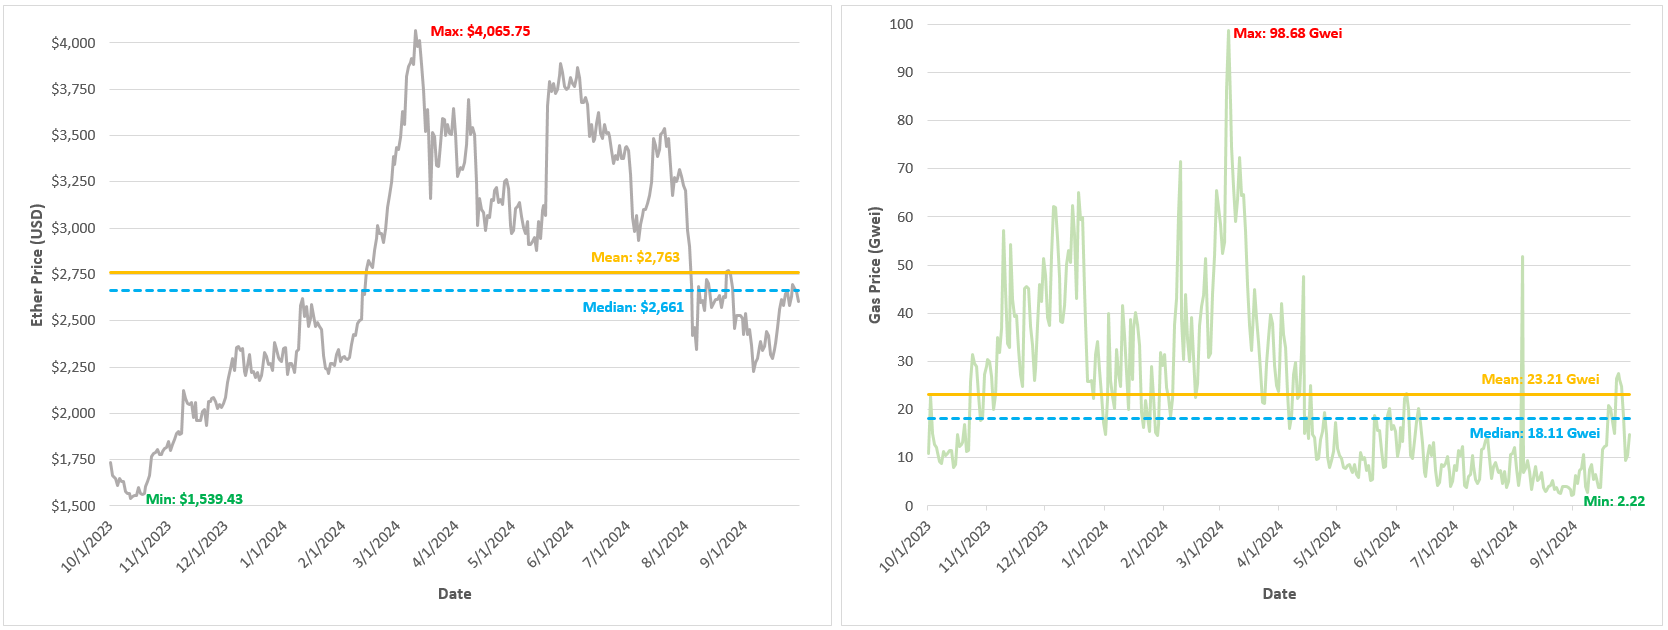
\includegraphics[width=\textwidth,keepaspectratio]{gas.png}
	\caption[Ethereum price and gas fluctuations]{Ethereum price in USD (left) and gas prices in Gwei (right) fluctuated from Sep-2023 to Sep-2024. Gas fluctuations were influenced by periods of high congestion or increased demand for transaction throughput. The maximum gas price during this period was 98.68 Gwei, recorded on March 5, 2024, while the minimum gas price was 2.22 Gwei on August 31, 2024 (source: \url{etherscan.io/chart}).}
	\label{fig:gas}
\end{figure}

\subsubsection{Rebalancing Cost}
To estimate daily rebalancing cost for LeverEdge, we need to break down the Ethereum gas costs based on the interaction with each application:
\begin{itemize}[leftmargin=*] 
	\item \textit{Interaction with Uniswap V3:} Swapping ETH to USDC involves a \texttt{swap} function, which typically costs around 120K to 180K gas depending on the liquidity conditions. We assume an average gas cost of 150K gas for the swap operation.
	
	\item \textit{Interaction with GMX:} The cost of interacting with the GMX protocol to buy and sell perpetual via USDC requires executing smart contract calls to open and close positions. These operations are relatively complex and typically consume around 300K to 400K gas per transaction. For the purpose of our analysis, we assume an average of 350K gas for a typical buy/sell transaction.
	
	\item \textit{Chainlink Keeper Network:} The keeper service triggers the rebalancing at a daily interval. The rebalancing trigger itself can vary, but Chainlink Keeper services typically use around 200K gas for basic triggers. Randomized delays add some variability as well. We assume 250K gas for each rebalancing trigger.
\end{itemize}
The total required gas is the sum of all interactions. Assuming the sequence of operations for a single rebalancing includes: (i) one Uniswap V3 swap for required conversions at 150K gas, (ii) one GMX buy/sell operation for perpetuals at 350K gas, and (iii) one Chainlink Keeper rebalancing trigger at 250K gas, the total gas consumption per day is \(150K + 350K + 250K = 750K\) gas unit. 

The cost of executing transactions on Ethereum Mainnet is influenced by network gas prices and the price of ETH in USD. As previously estimated, the average gas price is 23.21 and 0.09 Gwei on the Mainnet and Arbitrum, respectively. Therefore, the total cost of rebalancing for the required 750K gas, when ETH is priced at \$2,763, can be calculated as follows:
\begin{equation*}\label{eq:cost}
	\begin{aligned}
		\text{Mainnet rebalancing cost} & = \text{Gas units} \times \text{Gas fee} \times 10^{-9} \times \text{ETH price in USD} \\
		& = 750K \times 23.21 \text{ Gwei} \times 10^{-9} \times \$2,763 \\
		& = 0.0174075 \text{ ETH} \times \$2,763 = \$48.10 \text{ USD}		
	\end{aligned}
\end{equation*}
Thus, based on average gas price conditions, the estimated daily rebalancing cost is \$48.10 on the Mainnet. However, network congestion can lead to significant cost variations. As demonstrated in Figure \ref{fig:gas}, when the gas price on the Mainnet dropped to 2.22 Gwei, the daily cost decreased to just \$4.56, representing a 90\% reduction. Conversely, during congestion spikes, costs surged to as much as \$204.49, a 426\% increase when the gas price reached 98.68 Gwei. To mitigate these fluctuations, we have implemented specific techniques to reduce overall rebalancing expenses.

\paragraph{Employing MultiCall Transactions:} 
Bundling multiple operations into a single transaction can reduce costs by minimizing redundant gas expenditures that occur when each transaction is executed separately~\cite{hughes2021multicall}. Chainlink Keeper can trigger a single atomic bundle that executes all operations (Uniswap swap, dYdX/GMX Perps trade, and the rebalancing trigger itself) in one transaction. In this approach, all three operations share the transaction overhead costs (such as state updates and transaction initialization), further reducing the total gas consumption. Our analysis indicates that the 750K gas required for rebalancing can be reduced by an average of 14\% using MultiCall transactions.

\paragraph{Using L2 Chains:} 
L2 solutions reduce gas costs by enhancing transaction efficiency, batching multiple transactions, and leveraging Ethereum's Mainnet solely for security and final settlement~\cite{Gangwal_2022}. By consolidating many transactions and posting them to Ethereum as a single entry, they distribute gas costs across a larger number of users, lowering individual fees. This allows users to benefit Ethereum's robust security while paying only a small fraction of the gas fees compared to the Mainnet. 

\begin{example}
	On Ethereum Mainnet, the average cost for a token swap is approximately \$4.03, fluctuating between \$3.99 and \$4.54 depending on network congestion. In contrast, L2 networks like Arbitrum and Optimism can reduce these fees dramatically, often bringing the cost down to between \$0.09 and \$0.18 per swap~\cite{dailycoin2024}, representing more than 95\% savings in transaction costs.
\end{example}

LeverEdge implements a gateway contract on L1 to establish communication with the main contract on L2. This gateway is configurable and can connect to any L2 network where the main contract is deployed. We currently use Arbitrum and StarkEx, where active instances of GMX and dYdX already operate. dYdX offers perpetual contracts on various assets and is known for deep liquidity and zero gas fees. Comparatively, GMX provides low-cost, low-slippage trading on Arbitrum. While the zero gas fees on dYdX can fully eliminate rebalancing costs, issuers may still prefer GMX on Arbitrum due to its popularity among retail traders. In this case, the rebalancing cost would still be \(1-\frac{\$0.19}{\$48.10}=99.6\%\) cheaper than on the Mainnet.
\begin{equation*}
	\begin{aligned}
		\text{Arbitrum rebalancing cost} & = \text{Gas units} \times \text{Gas fee} \times 10^{-9} \times \text{ETH price in USD} \\
		& = 750K \times 0.09 \text{ Gwei} \times 10^{-9} \times \$2,763 \\
		& = 0.0000675 \text{ ETH} \times \$2,763 = \$0.19 \text{ USD}
	\end{aligned}
\end{equation*}

\section{Contributions}
The identified deficiencies in Chapter \ref{ch:shortfall} inspired us to consider possible solutions. We propose that operating on-chain mitigates most concerns (see Table~\ref{tab:solutions}) but building an on-chain LVT is non-trivial. The details of the design of LeverEdge are discussed through the following research questions:

\paragraph{RQ 1: What potential solutions could be proposed to address the current deficiencies of LVTs?} Implementing LVT on the blockchain can address these issues by bringing transparency to the total supply, transactions, holders, custody, auditing and financial backing. On-chain implementation should therefore be used by LVTs to mitigate the associated risks in centrally issued tokens. Although we proposed solutions for front-running, there would be still a possibility of front-running by miners who may intentionally include the rebalancing transaction in upcoming blocks and delay it to prioritize their own. Therefore, the risk of front-running can be alleviated and not completely eliminated. 

Some of the ways to reduce tracking error include: (i) increasing rebalancing frequency, possibly every \(n\) blocks instead of the default daily rebalancing, to more precisely maintain the target leverage ratio. This may involve using L2 chains that have lower transaction fees; (ii) performing interim rebalancing at threshold crossings of the underlying asset price (\eg \(\pm10\%\)), which would mitigate the impact of sudden price changes by rebalancing leverage more than once a day; and (iii) having a range allowing variation in leverage (\eg [1.95x, 2.05x] for a 2x long token), permitting small deviations without rebalancing. Thus, for both long and short tokens, this range must be set carefully to avoid major tracking errors. This approach should also be fully explained to investors to manage expectations properly, as it represents a workaround rather than a definitive solution.

Management fees in LVTs can be minimized by: (i) using advanced algorithms (iceberg or reverse orders), which enable the optimization of the timing and size of trades to minimize slippage and bid-ask spread costs; (ii) cross-trading between long and short funds, since issuers operating both can internalize trades by directly matching orders of funds sharing the same underlying assets. This internal matching at better prices further reduces slippage and transaction costs; (iii) using L2 chains~\cite{Gangwal_2022} in combination with MultiCall transactions~\cite{hughes2021multicall}, which further lower the cost.
	
\paragraph{RQ 2: What mitigation has been already done, and how far have these efforts been successful in eliminating the problems?} Even though there have been notable attempts to decentralize LVTs by FLI, Contango, Cube, Squeeth, Toros and TLX tokens, a closer look at their functionality shows ongoing shortcomings that need to be addressed. In this regard, we propose and evaluate a new L1-L2 hybrid model, LeverEdge, and compare how well it performs against others.
	
\paragraph{RQ 3: Can a new decentralized design, LeverEdge, succeed in effectively eliminating the existing shortcomings?} As shown in Table \ref{tab:compare}, most of the identified issues have been addressed in LeverEdge. But some inherent characteristics of the blockchain make it challenging to eliminate some issues completely, including: (i) the possibility of front-running cannot be fully addressed. Regardless of the technique used, ultimately miners have access to transactions and a malicious miner can prioritize its own transaction before the fund transaction. Therefore, in our design, the risk of front-running by other traders has been taken into account, (ii) to avoid frequent rebalancing and reduce costs, the rebalancing process can be delayed for minor deviations. For instance, the leverage of a 2x token can fluctuate in the range of [1.9x, 2.1x]. This range can be tightened, which increases the management fees of the token. Therefore, this is a trade-off between the fund's costs and the acceptable amount of deviation from the stated leverage, which is specific to the issuer.
	
\paragraph{RQ 4: How is the efficiency of LeverEdge on the Ethereum blockchain compared to the efficiency of existing decentralized LVTs?}  LeverEdge has addressed eight of the ten raised issues, and the other two are related to the nature of the blockchain and preference of the issuer, respectively. Our fully decentralized design is the first to deploy LVTs by utilizing decentralized perpetuals instead of debt or synthetic positions. This method addresses the shortcomings of centralized tokens and resolves issues in existing decentralized implementations. Key advantages :
\begin{itemize}
	\item Full ownership control for token holders through blockchain-based custody.
	\item Full transparency of total supply and transactions, recorded on the blockchain.
	\item Seamless interoperability with DeFi and availability for on-chain auditing.
	\item Verifiable financial backing via decentralized perpetual exchanges.
	\item Alleviation of front-running through randomized rebalancing, triggered by a decentralized autonomous network provided by Chainlink.
	\item Fixed leverage, with interim rebalancing to manage market volatility.
	\item Lower costs achieved through MultiCall transactions and L2 deployment.
\end{itemize}

\section{Discussion}
Leveraged tokens (LVTs) aim to mirror the advantages of leveraged ETFs (LETFs) seen in traditional markets. LVTs essentially combine the functionality of futures contracts or debt positions into a single token that can be traded on the spot market. Although they have the potential to result in significant profits, they also have the capability to increase potential losses. Despite involved risks, traders find LVTs appealing due to their simplicity, which removes the requirement for constant supervision of leveraged positions. In contrast to derivatives and margin trading, LVTs provide a less risky option with relatively modest returns, making them attractive to traders looking for a balanced risk-reward ratio.

Since 2019, over 1,600 leveraged tokens have been offered by various issuers. Previous research has identified ten key deficiencies in the technical and financial performance of these tokens. In this work, we review these issues and propose practical solutions. Decentralization stands out as the primary approach for resolving these deficiencies, along with enhancements to the internal algorithms governing the tokens. We also assess the performance of six decentralized tokens, identifying areas where further optimization is still needed.

To address these shortcomings, we introduce LeverEdge as a fully decentralized LVT, integrating the proposed solutions. Utilizing a hybrid L1-L2 architecture allows for seamless interaction with higher L1 liquidity while taking advantage of the faster execution and reduced fees on L2 chains. We evaluate LeverEdge in similar situations as other LVTs, demonstrating its capability to tackle the recognized flaws. It employs perpetual futures for generating leverage and incorporates a cross-chain mechanism for compatibility with various L2 ecosystems. Its design is focused on composability and deployed on the Ethereum blockchain. The open-source code has successfully passed security audits, serving as a blueprint for developing new decentralized LVTs or transitioning current centralized versions to decentralized options.